\section{Introduction}

During Run 1 of the CERN LHC data taking, a new particle consistent with the Higgs boson of the Standard Model (SM) was discovered \cite{Aad:2012tfa,Chatrchyan:2012ufa}.
The consistency of the new particle with the SM prediction implied that there may be new physics beyond the SM (BSM) at or around the electroweak scale.
As the Run 2 of the LHC started, the collision energy was significantly increased allowing for better reach for new physics and many direct searches have been performed with the Run 2 data.
However, so far no hints of direct evidence of new physics have been seen yet\footnote{For complete exclusion summary see: https://atlas.web.cern.ch/Atlas/GROUPS/PHYSICS/CombinedSummaryPlots/ and http://cms-results.web.cern.ch/cms-results/public-results/publications/}.

The new physics could be evading our current searches for a few reasons.
The new physics may be just beyond our current constraints in which case most likely will be conformed with the Run 3 data.
It could also be that new physics produce signatures that closely resemble known SM processes but with small rate and therefore becomes difficult in detecting.
Lastly, it is also possible that new physics is simply beyond the energy reach of the LHC.
If the new physics is beyond the energy reach of the LHC, then it will not be possible to directly produce a new particle at the LHC.
Instead, the effects of the new physics will manifest in the data through new interactions between known SM particles \cite{Weinberg:1978kz,Weinberg:1979sa,Buchmuller:1985jz}.
This is illustrated in Figure~\subref*{fig:TailIllustration} where the new degrees of freedom from a BSM model with mass $m_{X}$ that is larger than the LHC's collision energy $E_{\tiny\textrm{LHC}}$ is integrated out leaving only the interaction between known SM fields.

\begin{figure}[htb]
\centering
    \subfloat[When $m_{X} > E_{\tiny\textrm{LHC}}$ BSM effects show up in the tails instead of as a new resonance.]{
        \label{fig:TailIllustration}
        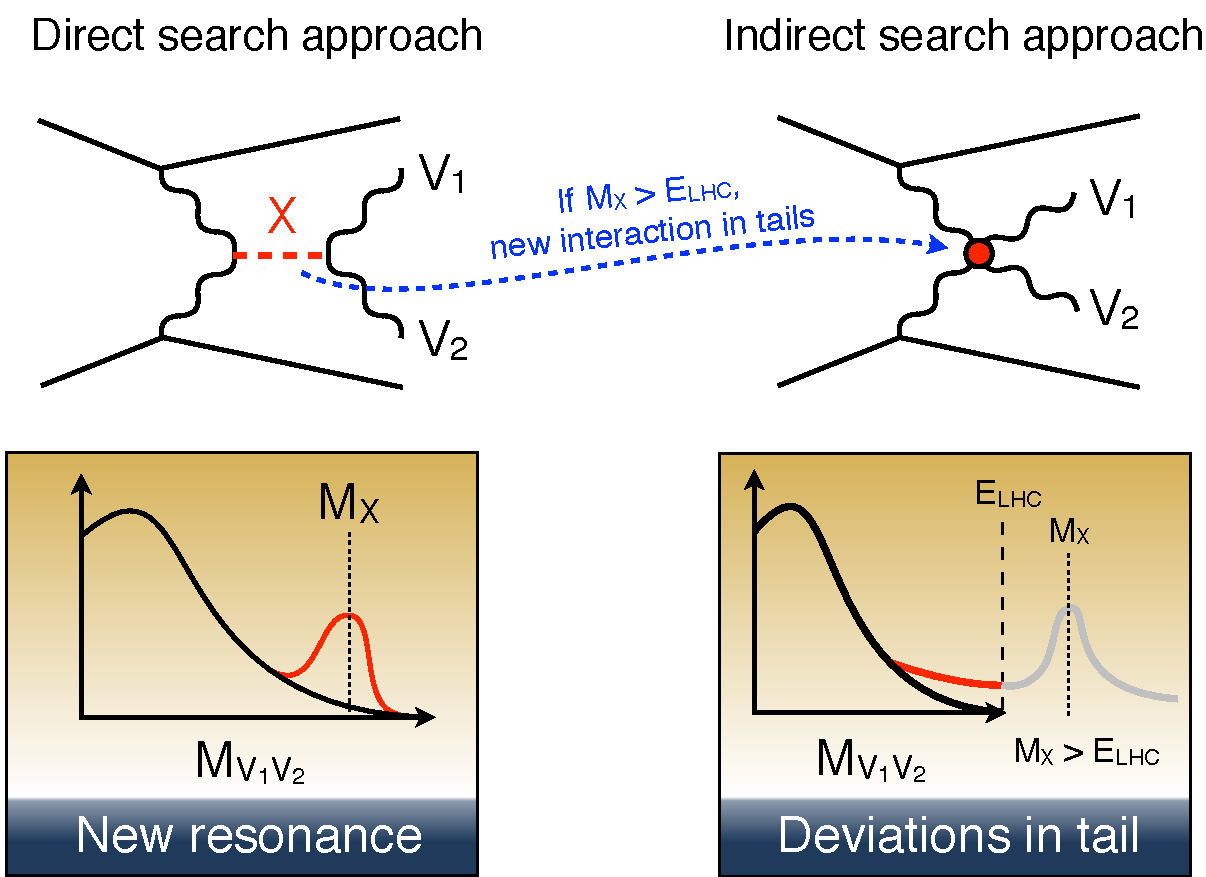
\includegraphics[height=2.2in]{TailIllustration.pdf}
        }
    \quad\quad
    \subfloat[SMEFT higher dimensional operators affecting high energy tails. Figure from \cite{Sirunyan:2019ksz} is taken to create the cartoon.]{
        \label{fig:SMEFTIllustration}
        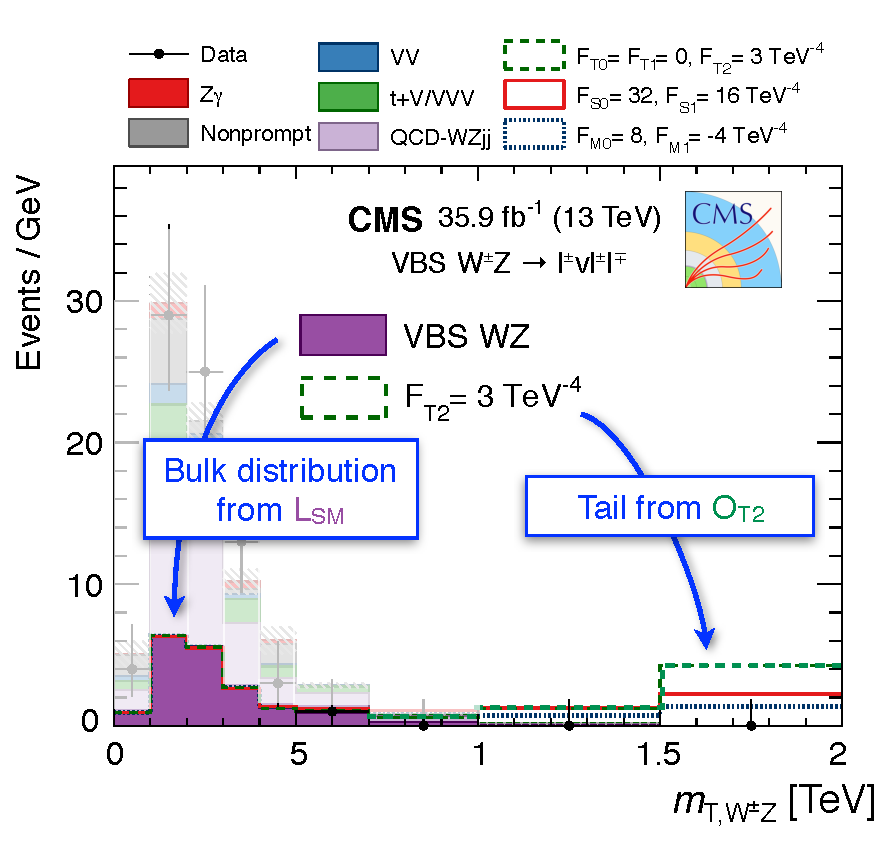
\includegraphics[height=2.2in]{SMEFTIllustration.pdf}
        }
\caption{Cartoon of BSM effects in the tails}
\label{fig:BSMTails}
\end{figure}

These possible new interactions can be systematically described by a framework called the SM Effective Field Theory (SMEFT) \cite{deBlas:2017xtg}.
In this framework, a set of higher dimensional operators constructed out of known SM fields are put together.
If there is a non-zero effect from one or some of the higher dimensional operators the effects will show up in the data as a deviation from the SM prediction.
Due to the dimensionality of these operators, the effects tend to be most pronounced in the tails of kinematic distributions, while the bulk of the kinematic distribution still roughly follows the SM prediction.
Therefore, searching for tails in kinematic distributions serve as a complementary approach to the more traditional bump hunt strategy.
It should also be noted that the bulk can also be modified by BSM models and hence measuring the bulk distribution also provides an essential confirmation of the SM.

Out of these higher dimensional operators, a handful of them predicts modifications to interactions between gauge bosons.
Therefore, SM processes involving multiboson interactions serve as an excellent testing ground to probe new physics.
As an example, a dimension-8 operator of the type,
\begin{equation}
    \mathcal{O}_{T2} = \textrm{Tr}\left[W_{\alpha\mu}W^{\mu\beta}\right]\times\textrm{Tr}\left[W_{\beta\nu}W^{\nu\alpha}\right],
\end{equation}
can lead to modifications in the distribution of the transverse mass of the $WZ$ system in the $pp\to WZjj$ process.
% increase in the tail distribution of the transverse mass of the $WZ$ system in the $pp\to WZjj$ process.
This can be seen from Figure~\subref*{fig:SMEFTIllustration} where the modification to the $m_{T,WZ}$ distribution from the $O_{T2}$ operator is highlighted in the dashed green line.
The effects are most visible in the \emph{rare} events in the tail with high energy and hence measuring the tail of such distributions can indirectly probe BSM physics.
Although not easily visible, the bulk distribution also gets modified but with a lesser degree.
Therefore, if a process at hand has a small cross section, simply observing the \emph{rare} process can also indirectly probe BSM physics.

There are many results from both ATLAS and CMS experiments related to the search or measurement of processes with multiboson interactions.
This proceeding will cover some of the recent highlights presented at the LHCP 2019.

\section{Studies of multiboson interactions in semi-leptonic final states}
\label{sec:diboson}

In general SM processes with multiboson interactions have small cross sections due to electroweak coupling constants.
Searches with fully-leptonic decay of the $VV$ ($V=W$ or $Z$) processes, therefore, have a cleaner signature with better sensitivity.
In fully-leptonic final states, often the process with the highest cross section is the signal itself, or other $VV$ processes with a relatively comparable cross section.
Final states with semi-leptonic decay of the $VV$ processes, on the other hand, have SM backgrounds from $V+$jets production, which have a much higher cross section, making it difficult to dig out the $VV$ signal process from the large $V+$jets background.

When considering BSM effects from higher dimensional operators, the picture changes.
Due to the smaller branching ratio of the $V$ bosons to leptonic final states, the number of expected high energy tail events for the fully-leptonic final states is significantly lower than that of the semi-leptonic final states.
In conjunction with the fact that the BSM effects can have a sizable enhancement at the tail of the distributions, studying the semi-leptonic final states can probe the BSM effects much further in the tail.
This is illustrated in Figure~\ref{fig:SemiLeptonicIllustration}.
The leptonic final states searches for rare diboson processes have already either established an observation ($>5\sigma$) or an evidence ($>3\sigma$) for the bulk distributions for various $VV+X$ processes \cite{Aaboud:2019nmv,Khachatryan:2014sta,Sirunyan:2017ret,Aad:2016ett,Aaboud:2018ddq,Sirunyan:2019ksz}.

\begin{figure}[htb]
\centering
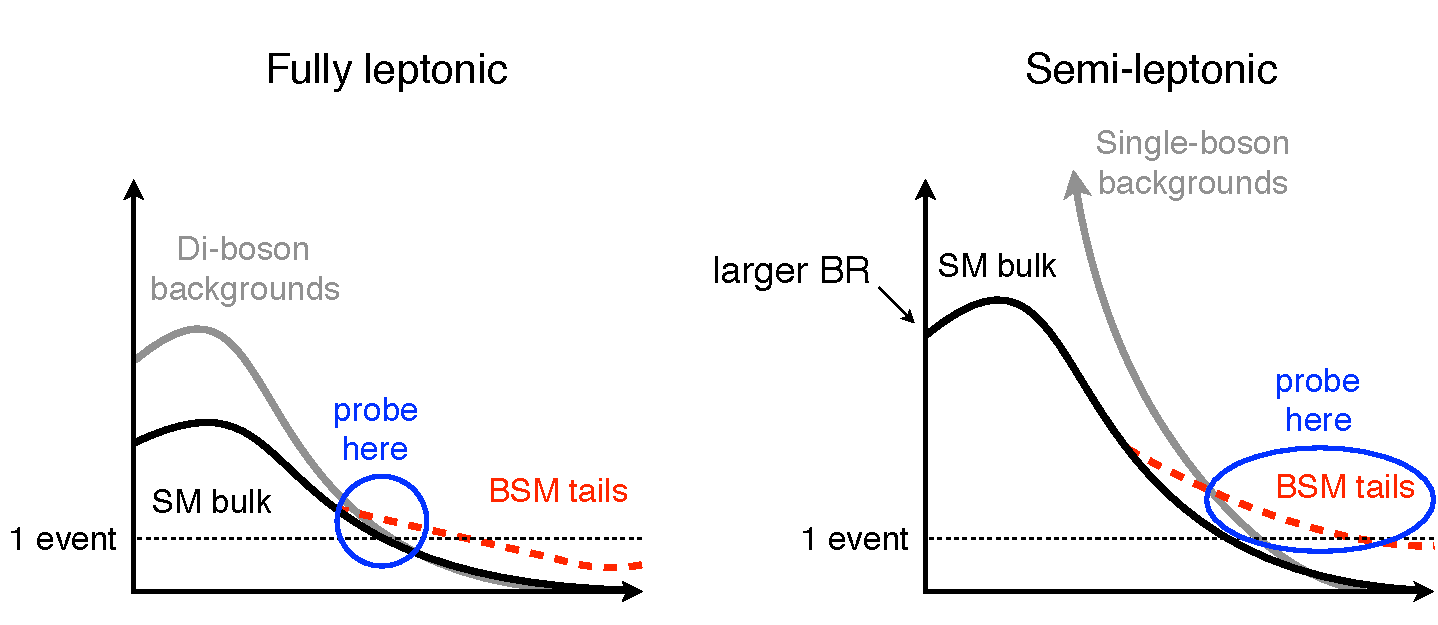
\includegraphics[height=2.0in]{SemiLeptonic.pdf}
\caption{Illustrating the complementarity between fully-leptonic and semi-leptonic final states.}
\label{fig:SemiLeptonicIllustration}
\end{figure}

\subsection{Studies of vector boson scattering processes in semi-leptonic final states}

The semi-leptonic final states searches with particular focus on the tail of the distribution have been done by the CMS experiment \cite{Sirunyan:2019der}.
The analysis targets signals produced via vector boson scattering (VBS).
The VBS processes have a characteristic signature where the accompanying jets (VBS jets) form a large invariant mass with a larger rapidity gap;
This search uses boosted techniques to tag the highly energetic hadronically decaying $V$ boson merging into a single fat-jet $J$.
The analysis was performed in one or two lepton final states targetting the processes such as $WV\to \ell\nu J$ or $ZV\to \ell\ell J$.
Figure~\subref*{fig:CMSVBSWV} shows the invariant mass of the $WV\to\ell\nu J$ system.
The BSM enhancement to the SM expectation is shown in the dashed line histograms.
Although the single $V+$jets processes at the bulk are very large as discussed previously, in the tail of the distribution with a high invariant mass of the $WV$ system, the BSM signal has non-zero expected yields and has a rate larger than that of the $V+$jets background.
This analysis placed limits on the higher dimensional operators (specifically the dimension-8 operators) and has one of the most stringent limits to date.

A similar search has been done in the ATLAS experiment as well \cite{Aad:2019xxo}.
ATLAS analysis has targetted not only the tail of the distribution with merged fat-jet but also the cases where the hadronically decaying $V$ leaves two resolved jets.
The analysis also targets one or two lepton final states. But, in addition, it targets zero lepton final states, where it targets $ZV\to \nu\nu J$ events.
Dedicated boosted decision tree (BDT) has been trained to enhance sensitivity to the rare signal over large $V+$jets background.
Figure~\subref*{fig:ATLASVBSWV} shows the BDT distribution for the two leptons plus a fat-jet final state.
This analysis also uses novel techniques designed to separate quark vs. gluon initiated jets.
This is particularly useful as the large $V+$jets backgrounds can be accompanied by both quark or gluon initiated jets while signal process events always contain only four quark initiated jets.
The signal regions are split into 9 different regions and the respective BDT distribution in each region is fitted simultaneously to extract the signal.
The observed and expected sensitivity is 2.7$\sigma$ and 2.5$\sigma$ respectively.

\begin{figure}[htb]
\centering
    \subfloat[]{
        \label{fig:CMSVBSWV}
        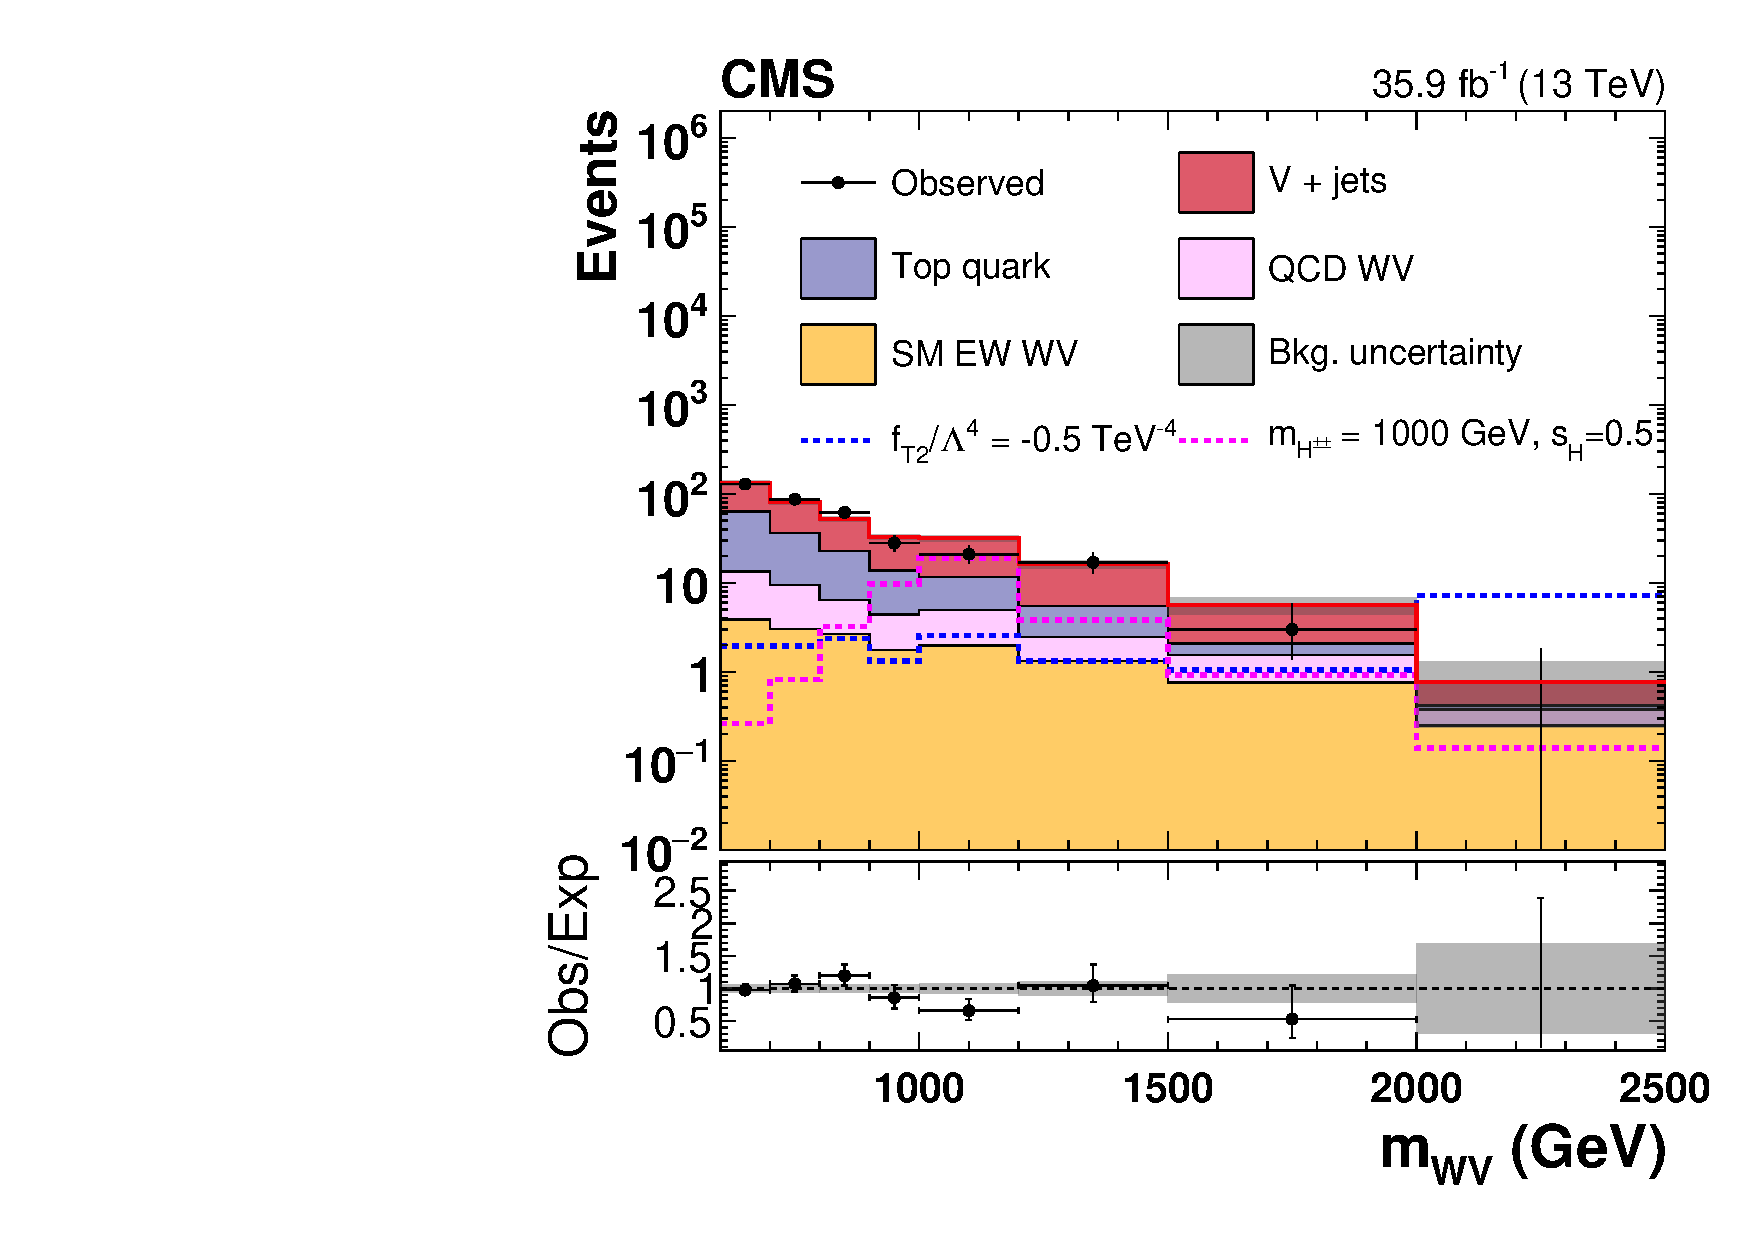
\includegraphics[height=2.4in]{CMS-SMP-18-006_Figure_004-a.pdf}
        }
    \quad\quad
    \subfloat[]{
        \label{fig:ATLASVBSWV}
        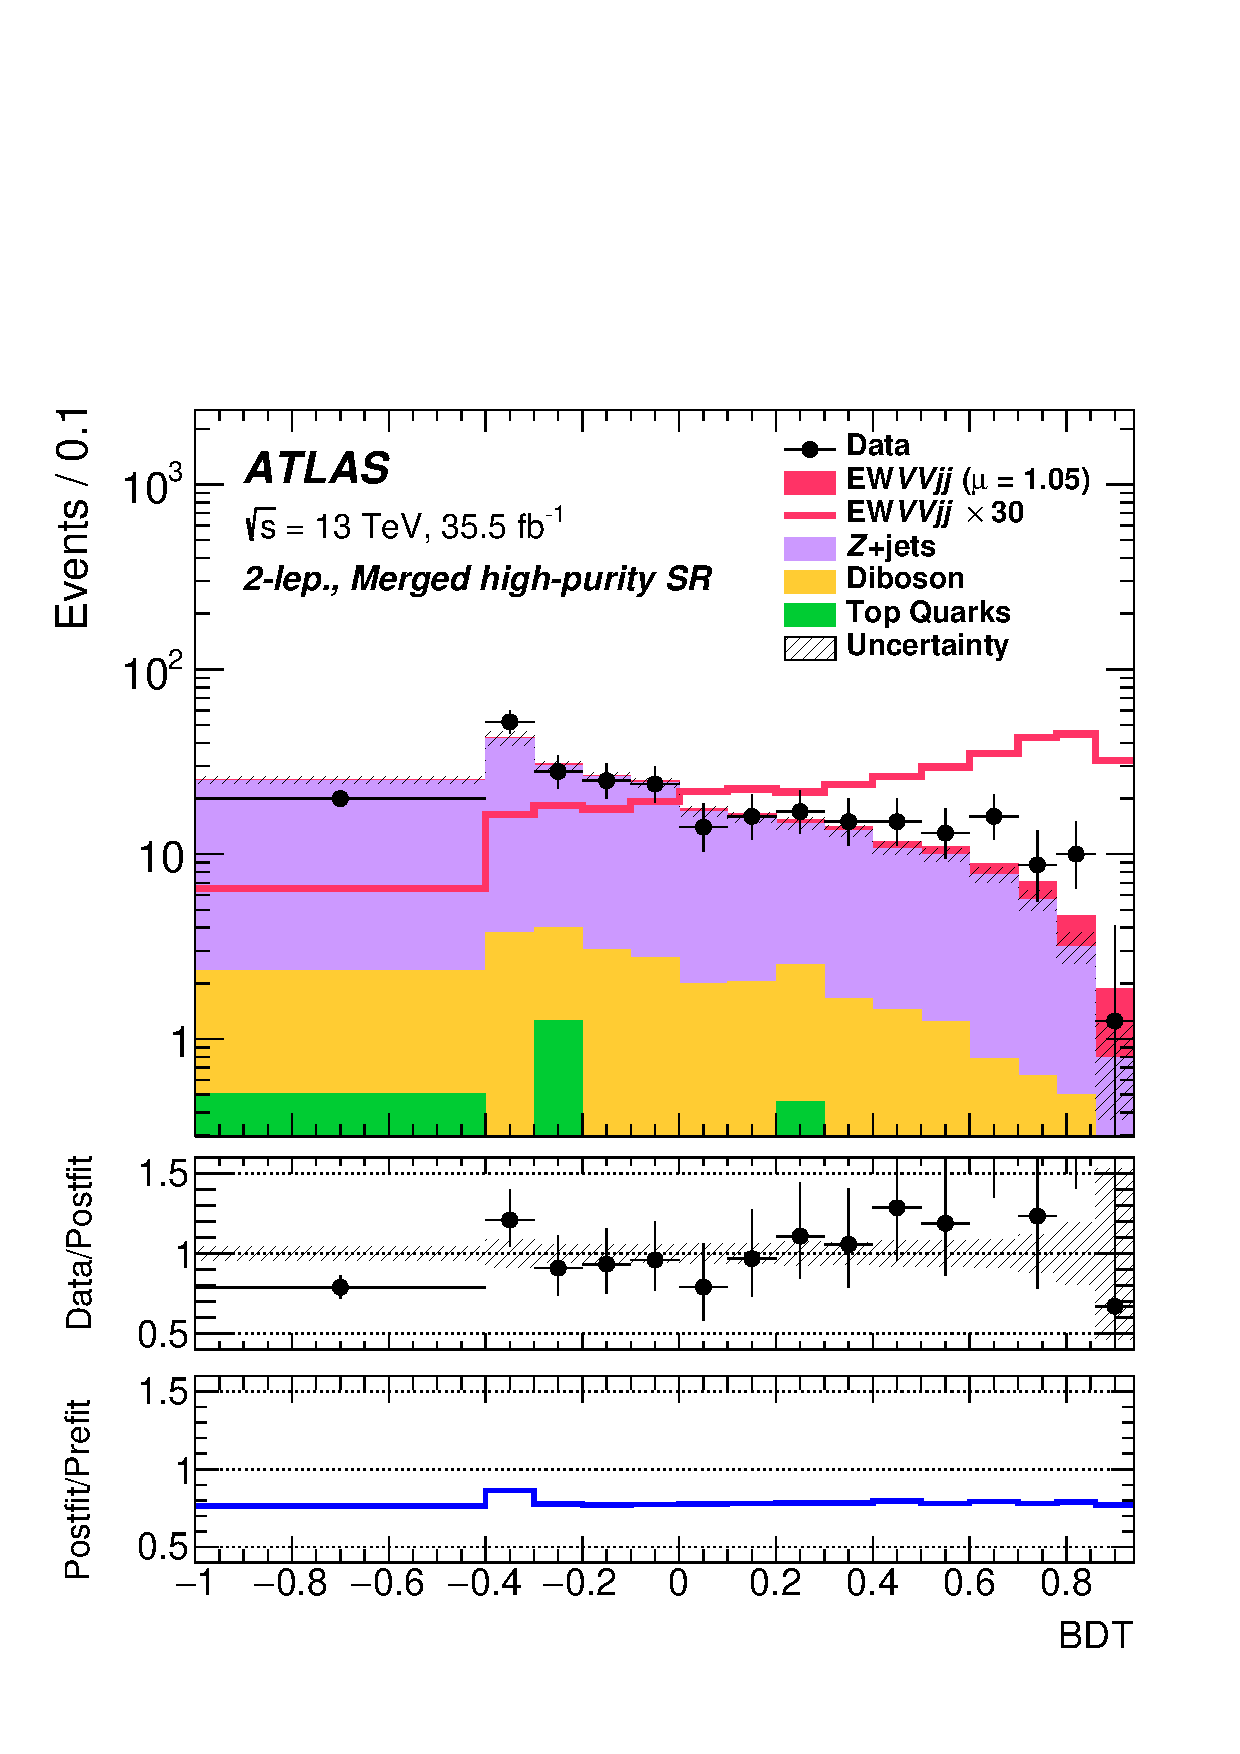
\includegraphics[height=2.4in]{fig_06a.pdf}
        }
\caption{Cartoon of BSM effects in the tails}
\label{fig:BSMTails}
\end{figure}

\subsection{Studies of diboson processes in semi-leptonic final states}
\label{sec:CMSWV}

\begin{figure}[htb]
\centering
    \subfloat[]{
        \label{fig:CMSWV}
        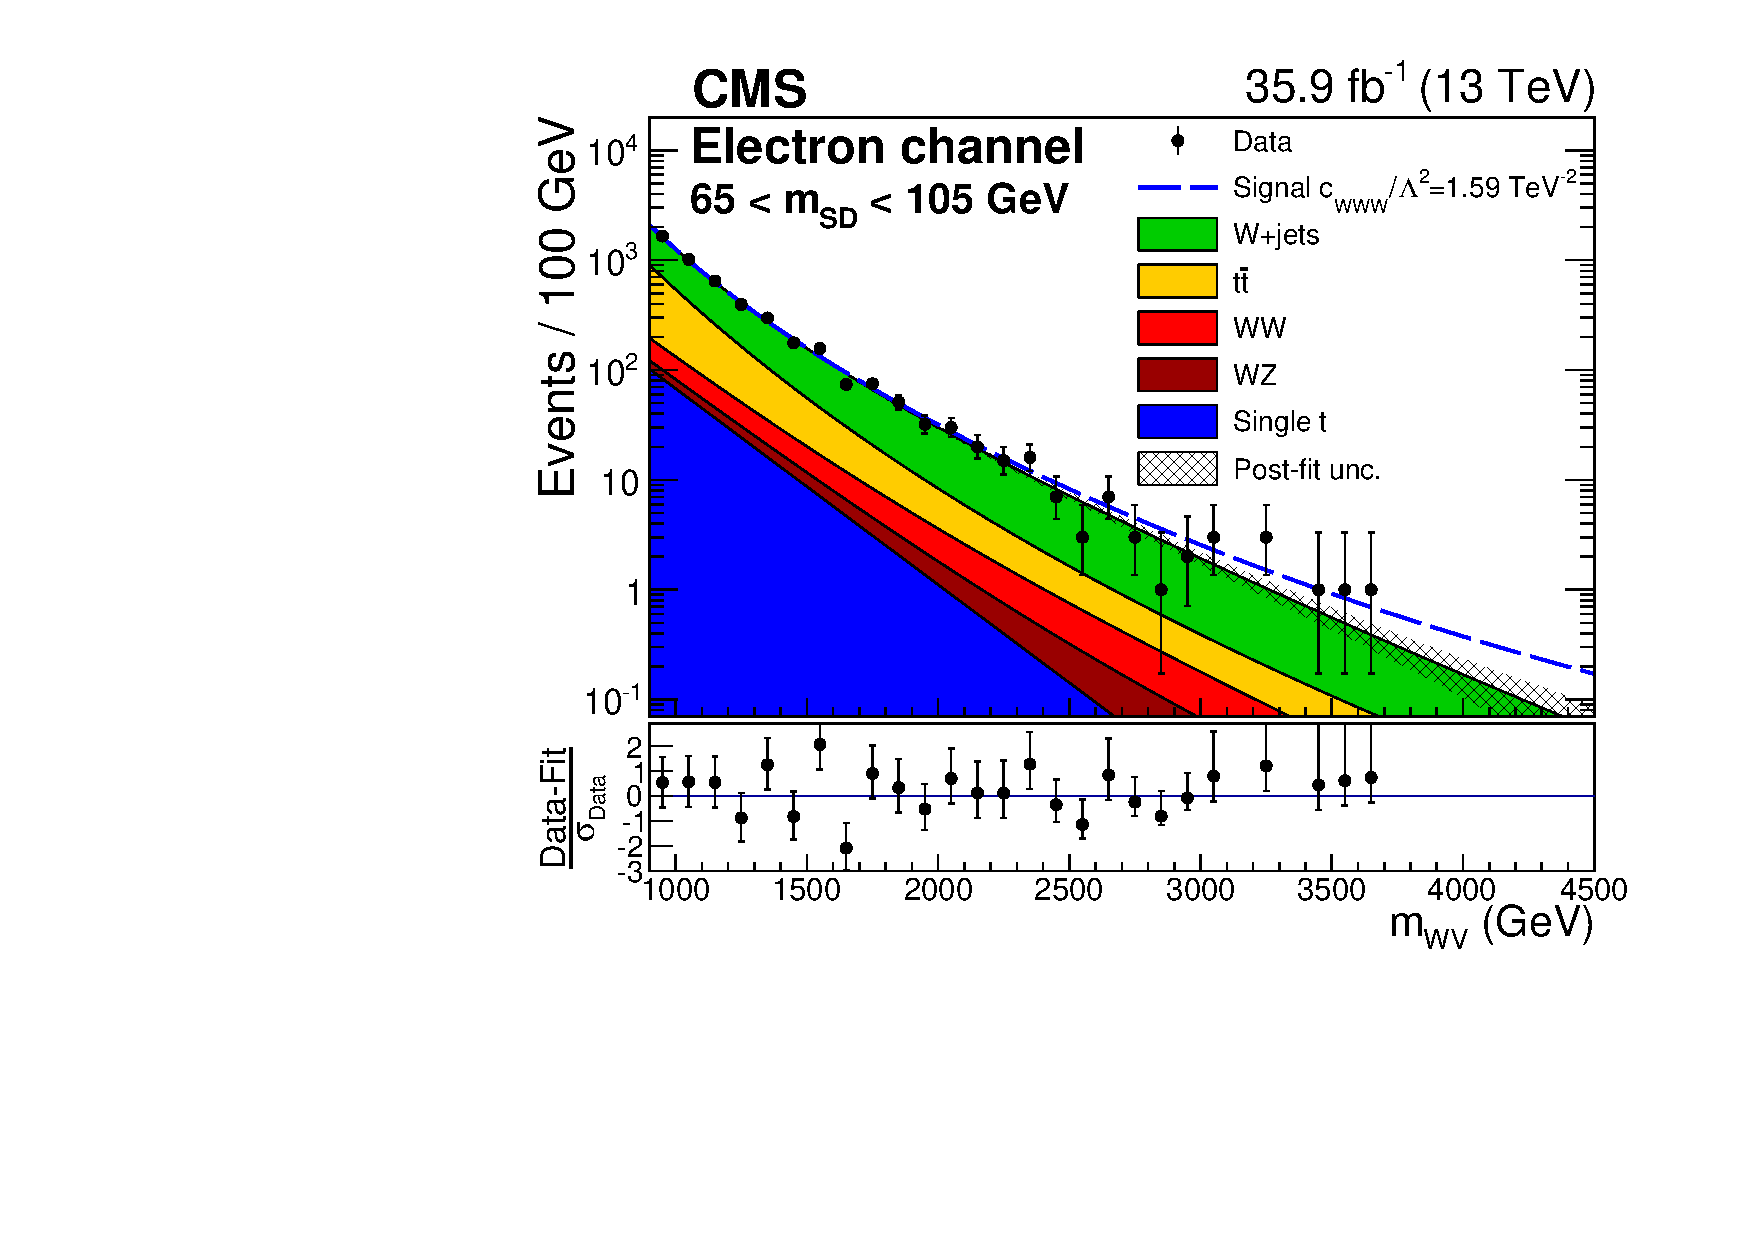
\includegraphics[height=2.2in]{CMS-SMP-18-008_Figure_004-c.pdf}
        }
    \subfloat[]{
        \label{fig:VBFWPtl}
        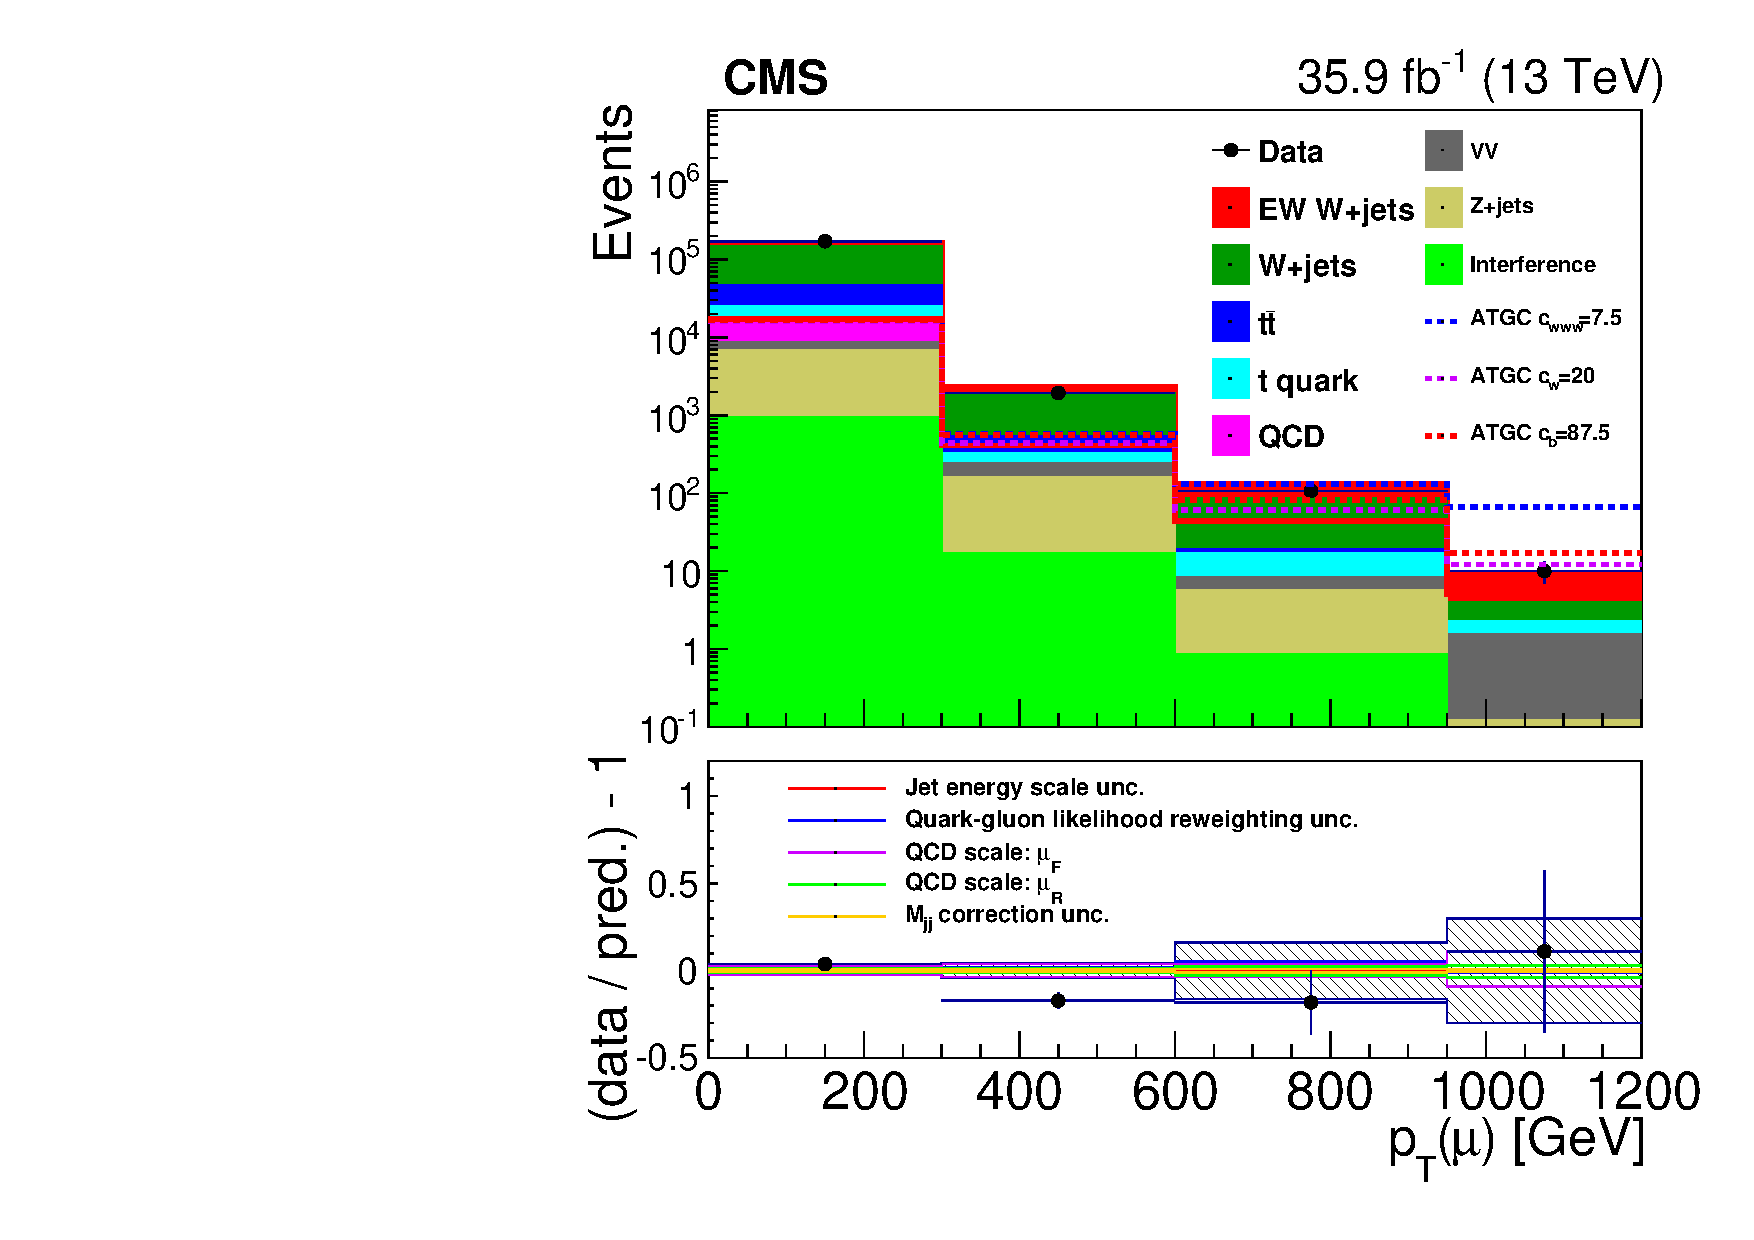
\includegraphics[height=2.2in]{CMS-SMP-17-011_Figure_010-a.pdf}
        }
\caption{}
\label{fig:BSMTails}
\end{figure}

CMS experiment also performed a search in semi-leptonic final states of diboson production involving triple gauge-boson couplings (TGCs) \cite{Sirunyan:2019gkh}.
The signal process is $pp\to VV$ without any VBS jets.
The analysis also utilizes boosted techniques to tag the merged fat-jet from a hadronically decaying $V$ boson.
Figure~\subref*{fig:CMSWV} shows the invariant mass distribution of the $pp\to WV\to e\nu J$ system.
Although the actual $pp\to WV$ process is well below the very large $W+$jets background process, starting around $m_{WV} > 2.5$~TeV the BSM effects from the higher dimensional operators become dominant over the $W+$jets.
Both the signal and the background distributions are parametrized using a series of exponential functions and fitted simultaneously to extract limits on the dimension-6 operators (viz. $\mathcal{O}_{WWW}$, $\mathcal{O}_{W}$, and $\mathcal{O}_{B}$).
The analysis is not sensitive to the SM rate of the $WV$ boson over a large $W+$jets background but places the most stringent limits on some of the dimension-6 operators to date.
The limits to the coefficients of the dimension-6 operators (represented as $c_{i} / \Lambda^2$) are shown in Table~\ref{tab:CMSWVLimits}.

\begin{table}[t]
\begin{center}
\caption{}
\label{tab:CMSWVLimits}
\begin{tabular}{l|ccc}
Operator coefficients & Expected limit & Observed limit & Observed best-fit \\ \hline
$c_{WWW} / \Lambda^2$ & [-1.44,1.47]   & [-1.58,1.59]   & -0.26  \\
$c_{W} / \Lambda^2$   & [-2.45,2.08]   & [-2.00,2.65]   & 1.21   \\
$c_{B} / \Lambda^2$   & [-8.38,8.06]   & [-8.78,8.54]   & 1.07   \\
\end{tabular}
\end{center}
\end{table}

\subsection{Single $W$ production via vector boson fusion}

Contrary to na\"ive expectation, the process $pp \to W jj$ involves multiboson interactions.
The Feynman diagram is the same as the process studied in Section~\ref{sec:CMSWV} except through crossing.
The production of single $W$ boson occurs through a fusion of the two $V$ bosons radiated from the incoming partons and hence is called vector boson fusion (VBF).
The accompanying jets (VBF jets) from the process also exhibits the same characteristics as the VBS jets.

CMS has performed an analysis targetting $pp \to W jj$ \cite{Sirunyan:2019dyi}.
A multivariate discriminant is trained using BDT method.
This analysis also utilizes a quark-gluon tagging technique in order to separate $W+$jets background from signal where the signal's VBF jets are always quark initiated jets.
The final BDT discriminant is fitted to extract the signal.
The analysis has established the signal with well over $>5\sigma$ significance.
The analysis then bins the events by the transverse momentum of the leptons $p_{T,\ell}$ and extract limits on dimension-6 operators.
Figure~\subref*{fig:VBFWPtl} shows the distribution of the $p_{T,\ell}$.
The effects from the dimension-6 operators are shown at the tail of the distribution as expected.
The limits to the dimension-6 operators are shown in Table~\ref{tab:CMSVBFWLimits}.
In the case for the dimension-6 operators $\mathcal{O}_{WWW}$, the constraint is weaker but comparable to the $pp \to WV$ analysis presented in Section~\ref{sec:CMSWV}, demonstrating complementarity between the two analyses.

\begin{table}[t]
\begin{center}
\caption{ place the caption here }
\label{tab:CMSVBFWLimits}
\begin{tabular}{l|cc}
Operator coefficients & Expected limit & Observed limit\\ \hline
$c_{WWW} / \Lambda^2$ & [-2.5,2.5]     & [-2.3,2.5]    \\
$c_{W} / \Lambda^2$   & [-16,19]       & [-8.8,1.6]    \\
$c_{B} / \Lambda^2$   & [-62,61]       & [-45,46]      \\
\end{tabular}
\end{center}
\end{table}
\section{Triboson production}

The couplings between the gauge bosons are fully determined by the non-Abelian gauge structure of the theory, namely the $\textrm{SU}(2)_\textrm{L} \times \textrm{U}(1)_\textrm{Y}$.
Therefore, measurements of triboson productions are sensitive to the TGCs and the QGC between the massive bosons (i.e. $W$ or $Z$).
As discussed in Section~\ref{sec:diboson} multiboson interactions have been established through various measurements and therefore it necessarily implies that there are additional contributions to the production process of triboson final states through TGCs and QGCs.

Figure~\ref{fig:feynman} shows the tree-level diagrams of the production of three massive bosons.
From the figure, it can be seen that in addition to the diagram with gauge bosons radiating off from quark lines, there are diagrams involving TGCs and QGCs.
In addition, the recent Higgs boson discovery \cite{Aad:2012tfa,Chatrchyan:2012ufa} and subsequent measurements on its $VVH$ couplings \cite{Sirunyan:2018egh,Chatrchyan:2013iaa,Sirunyan:2019twz,Chatrchyan:2013mxa,Aaboud:2018jqu,Aaboud:2017vzb,ATLAS:2014aga,Aad:2014eva}, which confirms the couplings between the newly found scalar boson and massive gauge bosons, further implies that the triboson production of massive bosons should also occur in $pp$ collisions via the newly found scalar particle.
This is also illustrated in Figure~\ref{fig:feynman} through the triboson production diagram via $VVH$ couplings.
Therefore, direct observations of the triboson productions of three massive bosons serve as essential confirmations of the SM predictions.

\begin{figure}[thb]
\begin{center}
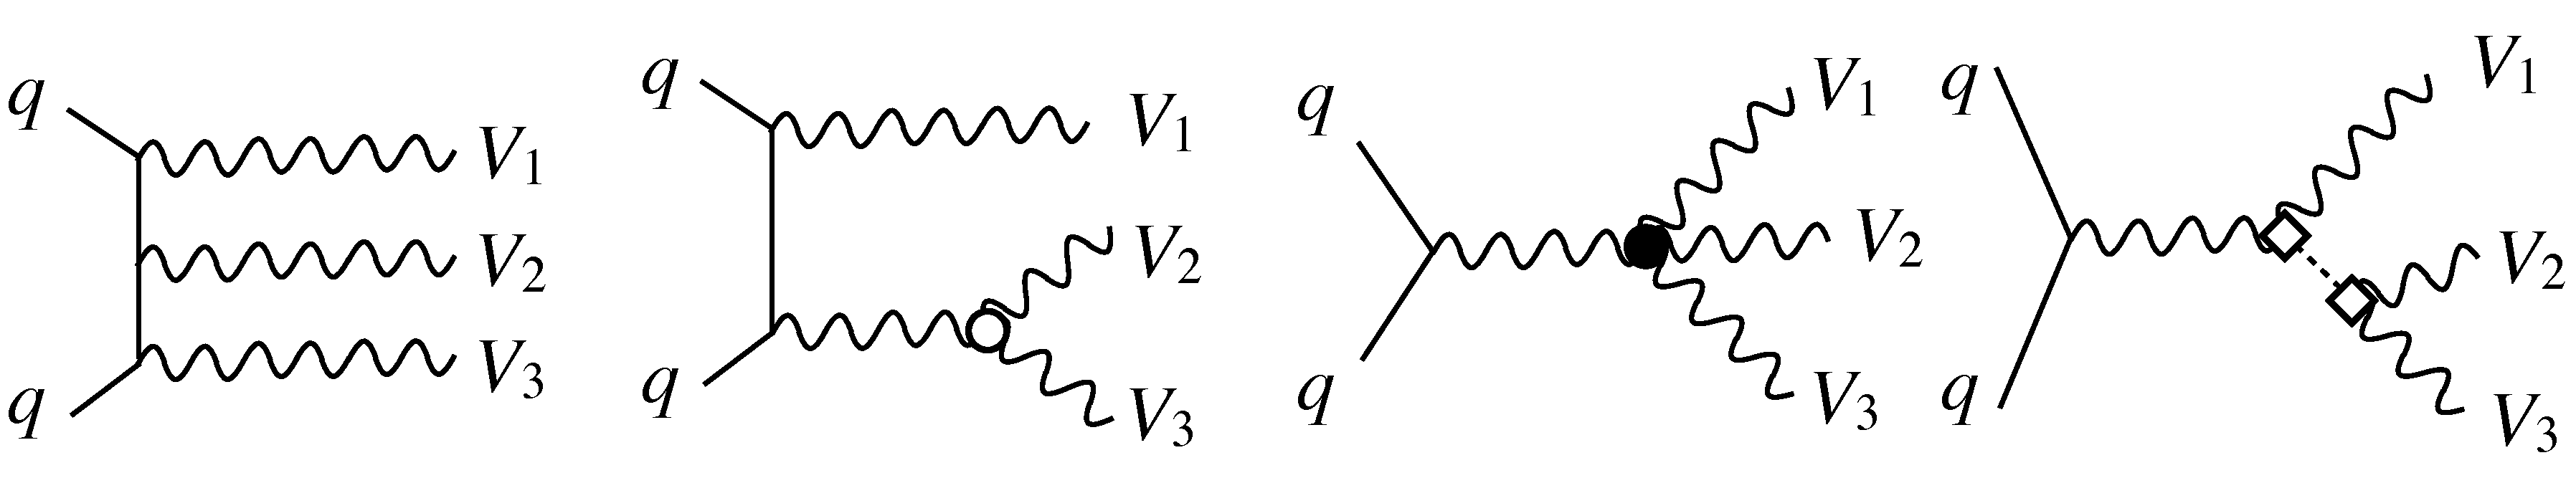
\includegraphics[width=0.8\textwidth]{FeynmanDiagram.pdf}
\caption{
\label{fig:feynman}
Tree-level Feynman diagrams of three boson productions ($V_{i} = W, Z$), where the triple gauge-boson coupling, quartic gauge-boson coupling, and $VVH$ couplings are marked by $\circ$, $\bullet$, and $\diamond$, respectively.
}
\end{center}
\end{figure}

CMS has performed an analysis in the search for the WWW production process \cite{CMS:2019mpq}.
The analysis was performed in the same-charge dilepton final states (SS) and trilepton final states.
When the signal events decay into the SS final states, the remaining W must decay hadronically which can be tagged via identifying the two jets from its decay.
The analysis, therefore, separates events based on whether the hadronically decaying W is tagged or not.
The selected events are further separated based on the lepton flavors.
A total of nine signal regions was fitted simultaneously to extract the signal.
The yields in each signal regions are shown in Figure~\subref*{fig:CMSWWWSM}.
The observed and expected sensitivity is 0.6$\sigma$ and 1.8$\sigma$ respectively.
The $S_{T}$ distribution, defined as the scalar sum of all the transverse momentum of the objects in the event, is fitted to extract the limits on the dimension-8 operators.
As seen in Figure~\subref*{fig:CMSWWWEFT}, the BSM tail events are expected to dominate at the high tail of $S_{T}$ distributions.
The limits on the dimension-8 operators placed from the analysis are shown in Table~\ref{tab:CMSWWWLimits}.

\begin{figure}[htb]
\centering
    \subfloat[]{
        \label{fig:CMSWWWSM}
        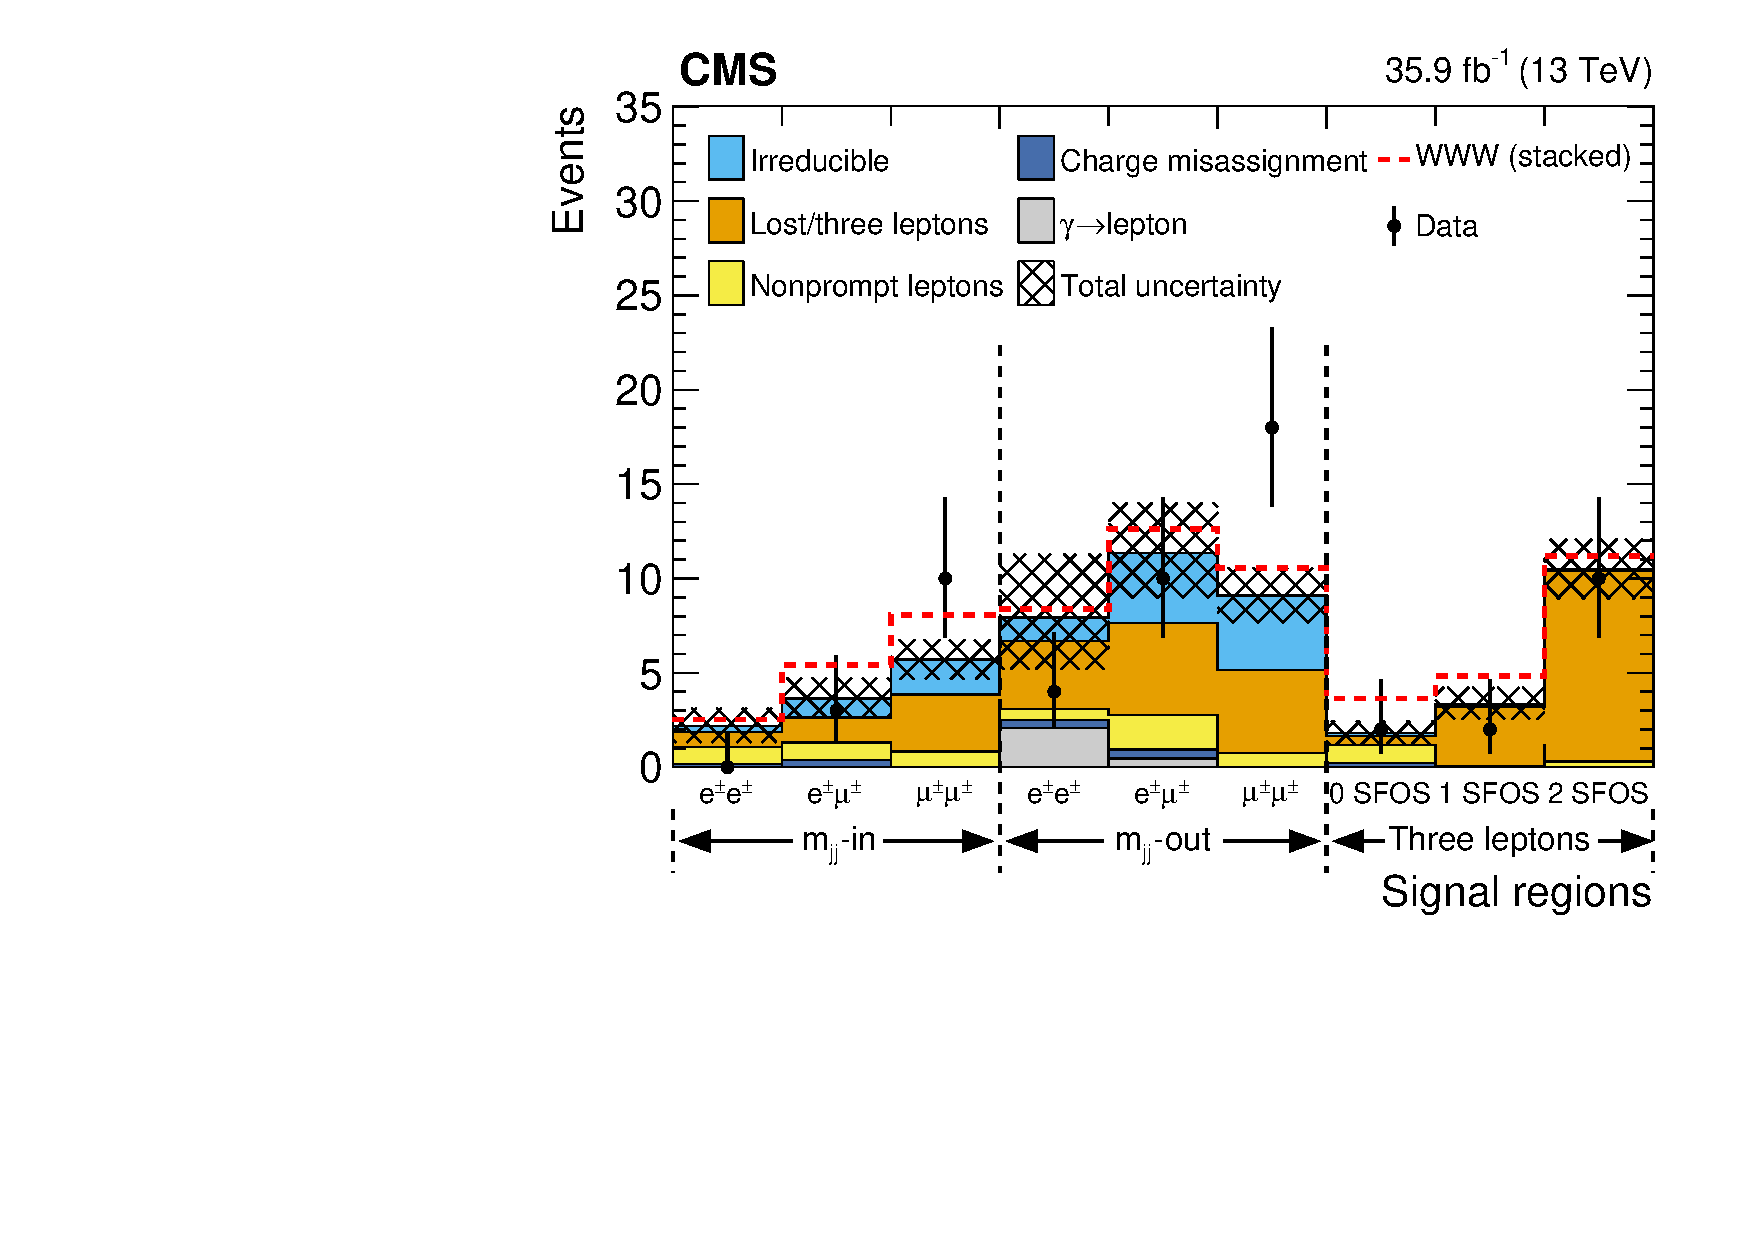
\includegraphics[width=0.5\textwidth]{CMS-SMP-17-013_Figure_002.pdf}
        }
    \subfloat[]{
        \label{fig:CMSWWWEFT}
        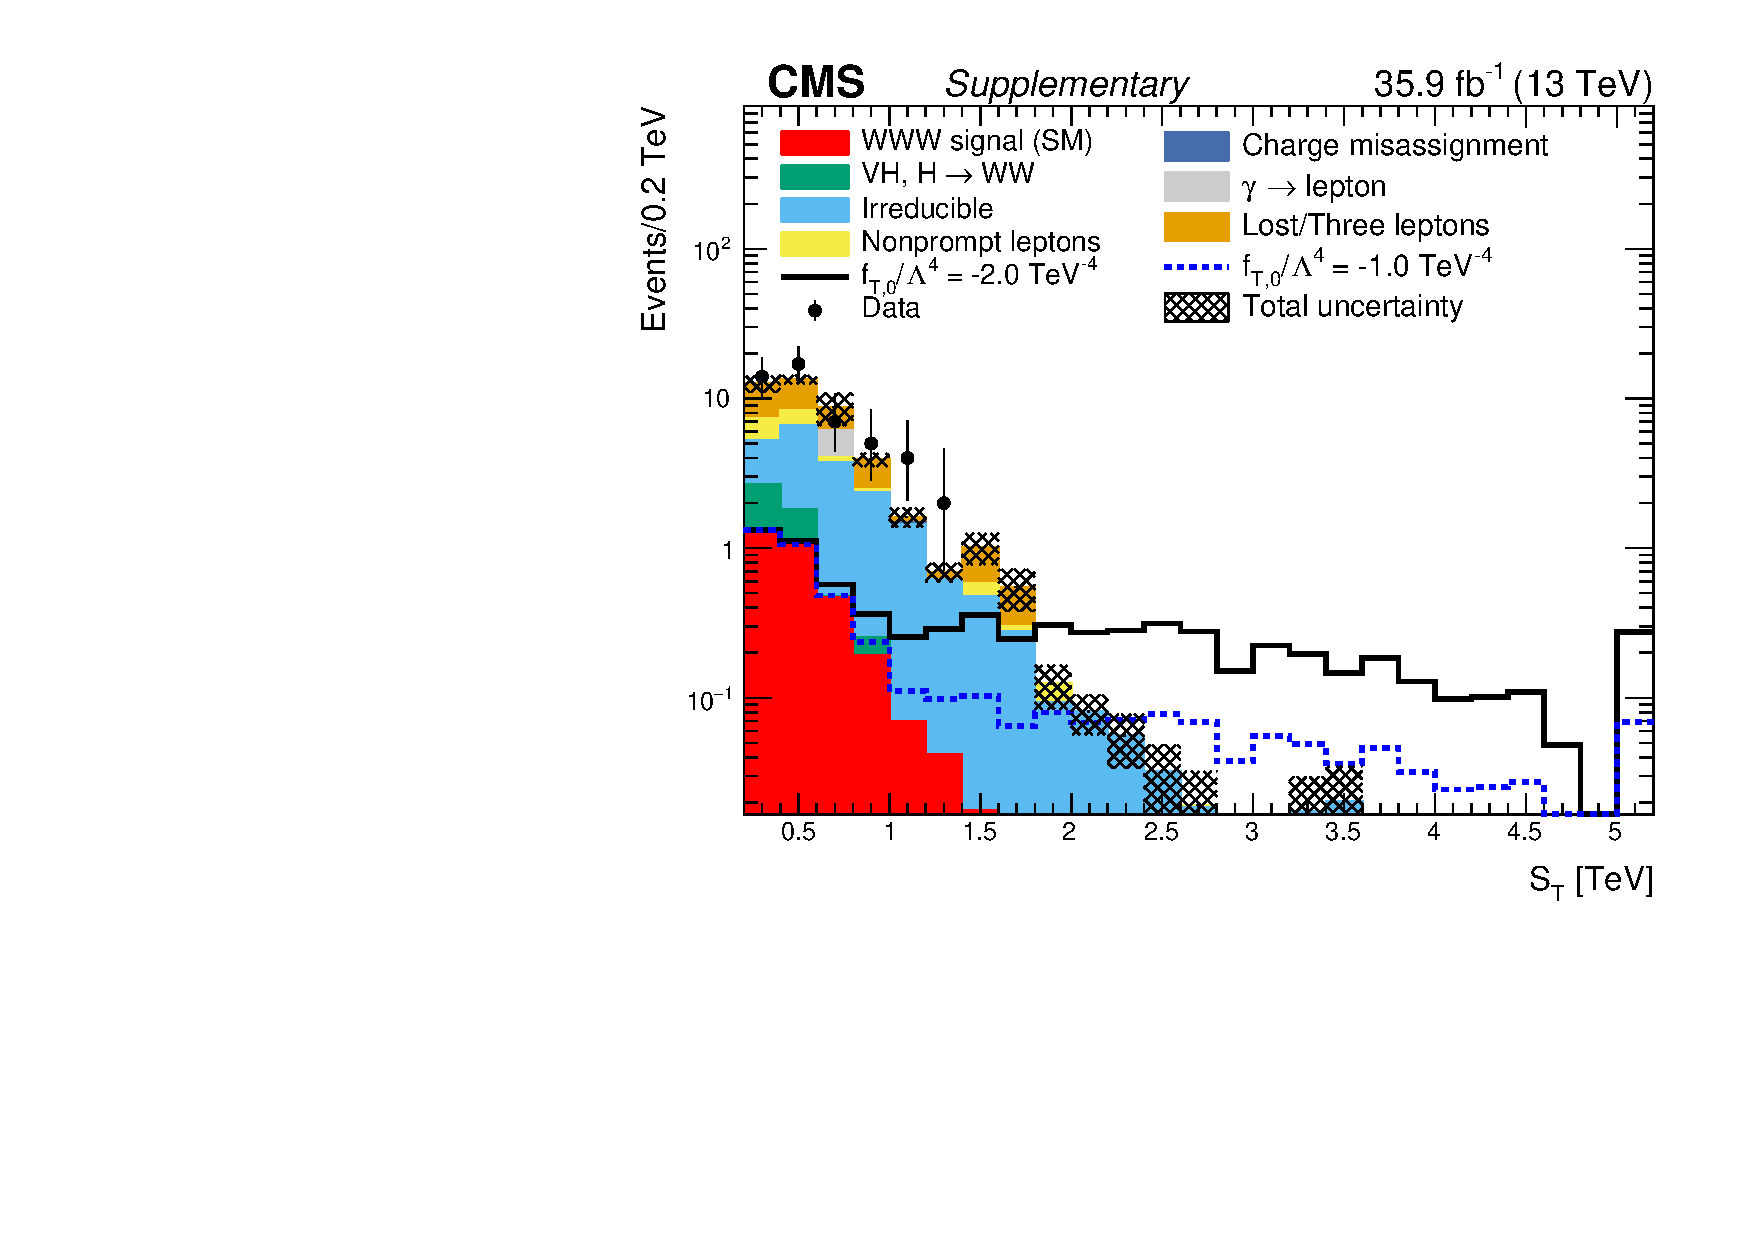
\includegraphics[width=0.5\textwidth]{CMS-SMP-17-013_Figure-aux_004.pdf}
        }
\caption{}
\label{fig:CMSWWW}
\end{figure}

\begin{table}[t]
\begin{center}
\caption{ place the caption here }
\label{tab:CMSWWWLimits}
\begin{tabular}{l|cc}
Operator coefficients & Expected limit & Observed limit\\ \hline
$f_{T,0} / \Lambda^2$ & [-1.3,1.3]     & [-1.2,1.2]    \\
$f_{T,1} / \Lambda^2$ & [-3.7,3.7]     & [-3.3,3.3]    \\
$f_{T,2} / \Lambda^2$ & [-3.0,2.9]     & [-2.7,2.6]    \\
\end{tabular}
\end{center}
\end{table}

ATLAS has performed an analysis in the search for the triboson production process as well \cite{Aad:2019udh}.
The search takes all three WWW, WWZ, and WZZ as the signal process.
The SS final states, trilepton final states, and four-lepton final states have been studied.
Events in the SS final states are fitted by the two jets in the events designed to tag the hadronically decaying W.
Figure~\subref*{fig:ATLASVVVSS} shows the dijet invariant mass distributions of the two jets tagged as coming from hadronically decaying W.
The distribution exhibits a peak around the W mass indicating a presence of the signal.
For the four-lepton final states analysis, dedicated BDTs are constructed to extract the signal.
Figure~\subref*{fig:ATLASVVV4L} shows the BDT distribution in the final states with a pair of same-flavor lepton tagged as originating from Z plus an opposite-charge pair of $e\mu$ events.
The region exhibits high purity to the signal.
The signal strength for the $VVV$ process is extracted by simultaneously fitting all the distributions in different lepton final states.
Figure~\subref*{fig:ATLASVVVMu} shows the signal strengths for different signal regions and the combined signal strength.
The observed signal strength is $\mu = 1.40^{+0.39}_{-0.37}$ and the observed (expected) significance is 4.0$\sigma$ (3.1$\sigma$).

\begin{figure}[htb]
\centering
    \subfloat[]{
        \label{fig:ATLASVVVSS}
        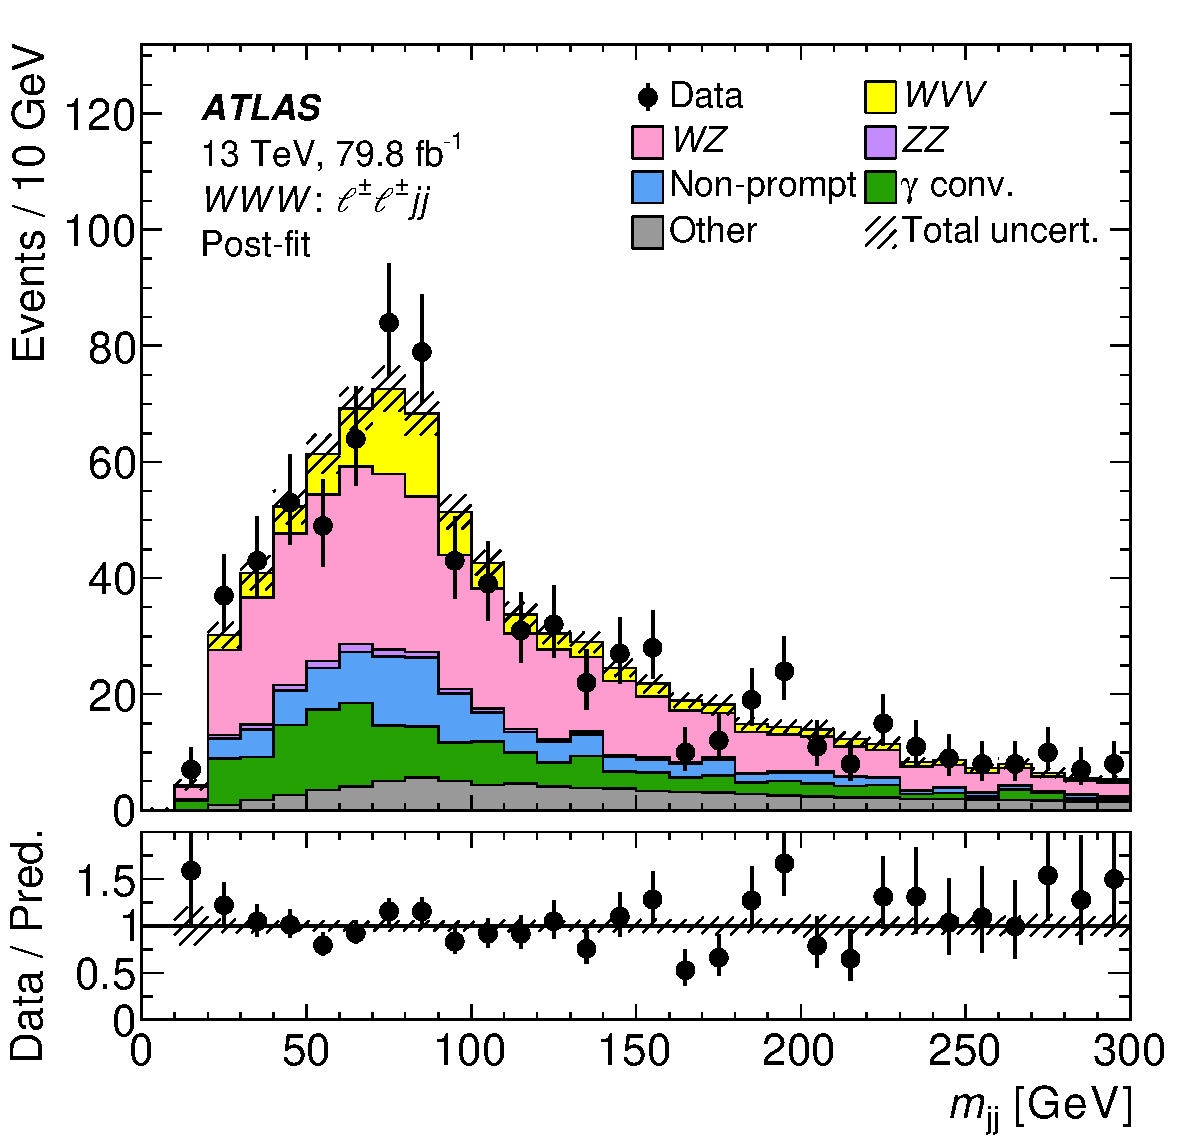
\includegraphics[width=0.30\textwidth]{fig_04a.pdf}
        }
    \subfloat[]{
        \label{fig:ATLASVVV4L}
        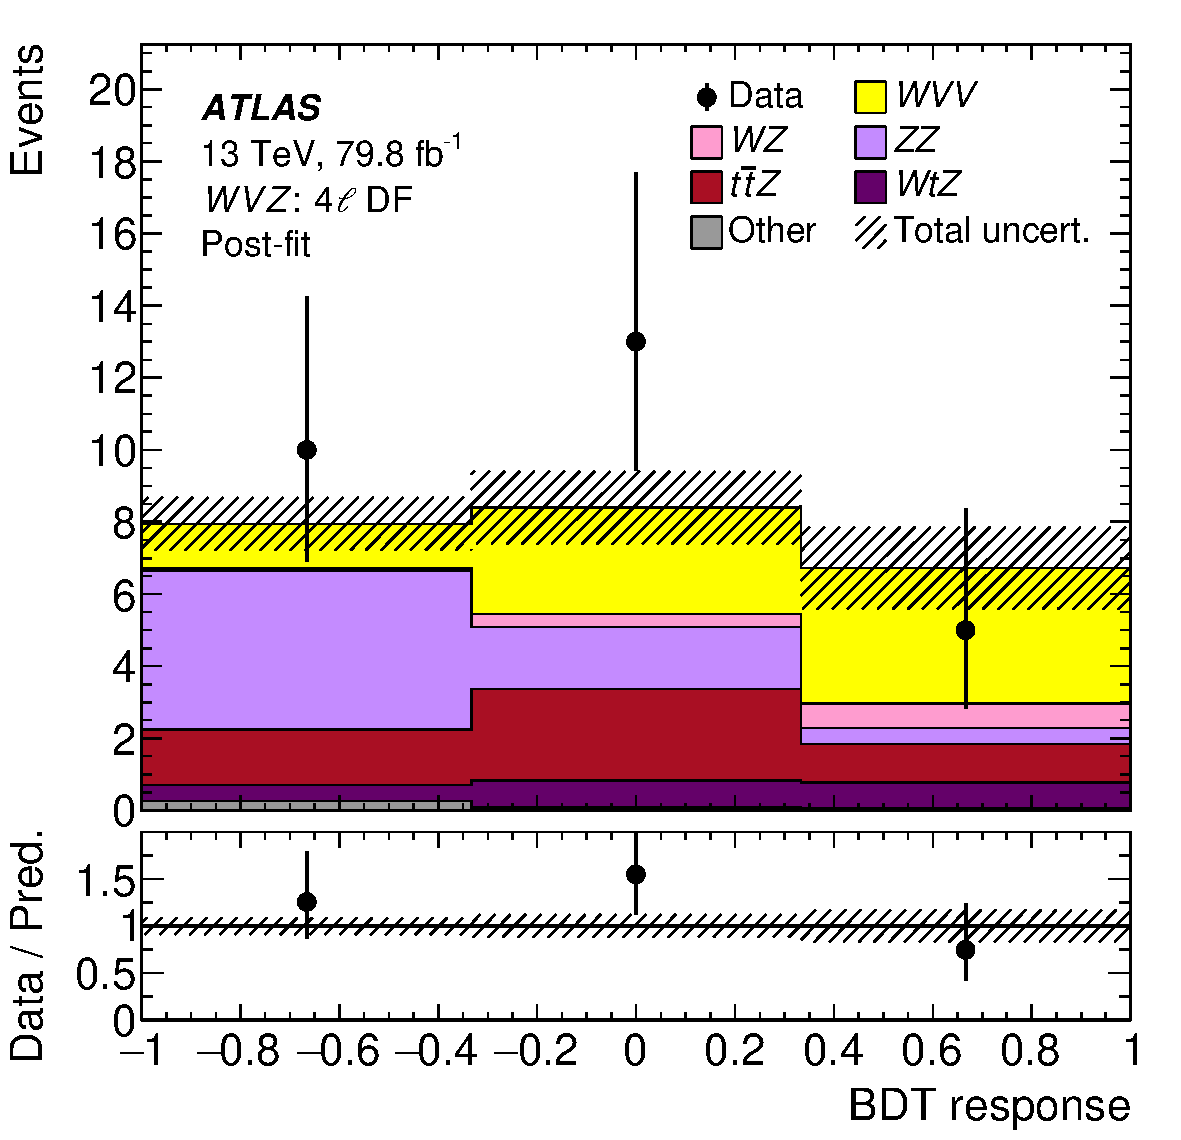
\includegraphics[width=0.30\textwidth]{fig_04d.pdf}
        }
    \subfloat[]{
        \label{fig:ATLASVVVMu}
        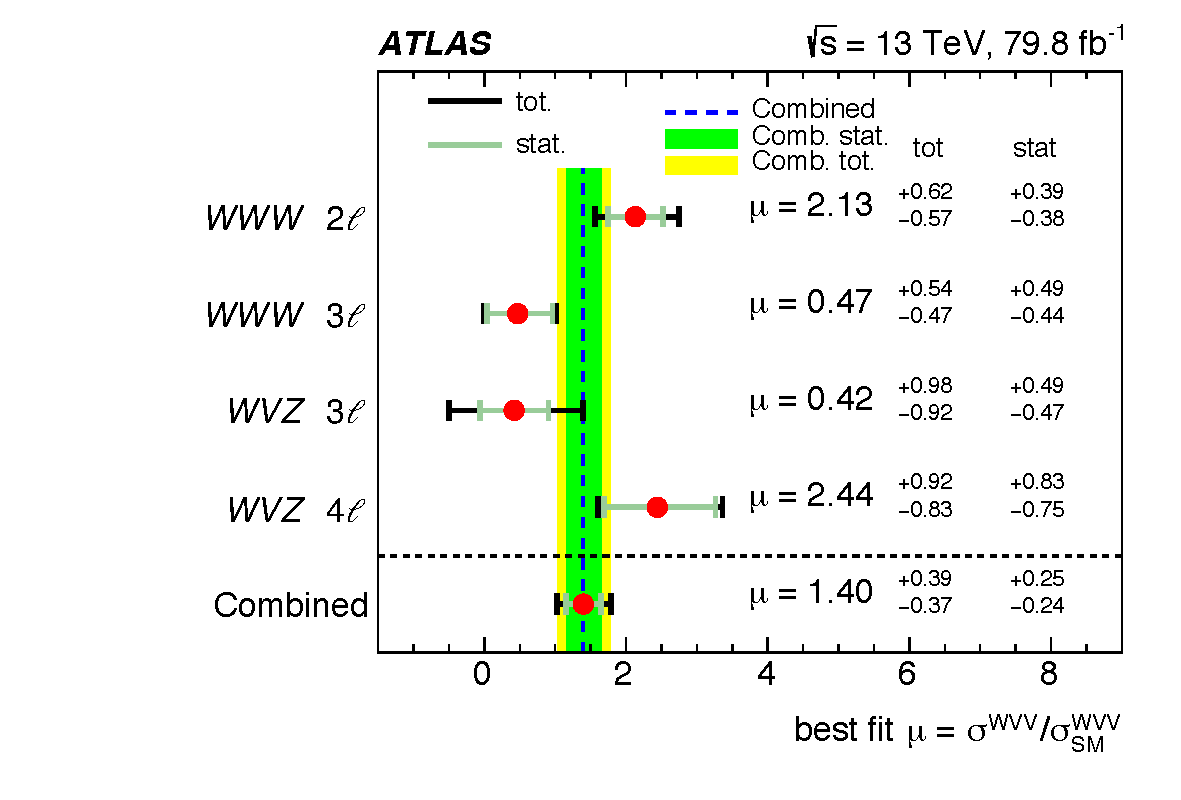
\includegraphics[width=0.40\textwidth]{fig_06a_vvv.pdf}
        }
\caption{}
\label{fig:ATLASVVV}
\end{figure}

\section{Future prospects}

The upcoming high luminosity LHC (HL-LHC) program to run at an unprecedented level of instantaneous luminosity.
The projected number of integrated luminosity is 3$\textrm{ab}^{-1}$.
It will allow for the rare processes discussed in previous sections to be accessible at much higher precision.
Many of the SM processes that are currently being established with either $3$ or $5\sigma$ will be probable at a few percent levels and HL-LHC will allow both ATLAS and CMS collaboration to measure differential cross section measurements.
There are many projection studies made in regards to SM processes with multiboson interactions \cite{Atlas:2019qfx}.
We will discuss one example in this proceeding from the myriad of studies.

One of the important questions that arose after the discovery of the Higgs boson is whether the newly found particle is \emph{the} SM Higgs boson.
Whether the newly discovered boson preserves unitarity of the VBS amplitude at all energies, or new other processes are involved is still unknown \cite{Veltman:1976rt,Lee:1977yc,Lee:1977eg}.
In particular, measuring the differential cross section of $pp\to W_{L}^{\pm}W_{L}^{\pm}jj$, where $W_{L}$ indicates longitudinally polarized W boson, is noted as one of the most crucial test of the SM prediction and both ATLAS and CMS experiments have studied projected sensitivity with the expected amount of data set from the HL-LHC program.

Disentangling longitudinally polarized W boson from transversely polarized W boson is not easy.
One of the discriminating variables is the opening angle between the two VBS jet $|\Delta\phi_{jj}|$.
Fitting on the distribution of the $|\Delta\phi_{jj}|$ one can extract the longitudinally polarized WW scattering process cross section.
Results for the expected significances as a function of integrated luminosity is presented in Figure~\ref{fig:VBSWWFuture}.
With the full HL-LHC data set, the expected sensitivity ranges between 1.7$\sigma$ to 2.7$\sigma$.

\begin{figure}[htb]
\centering
    \subfloat[]{
        \label{fig:VBSWWFutureCMS}
        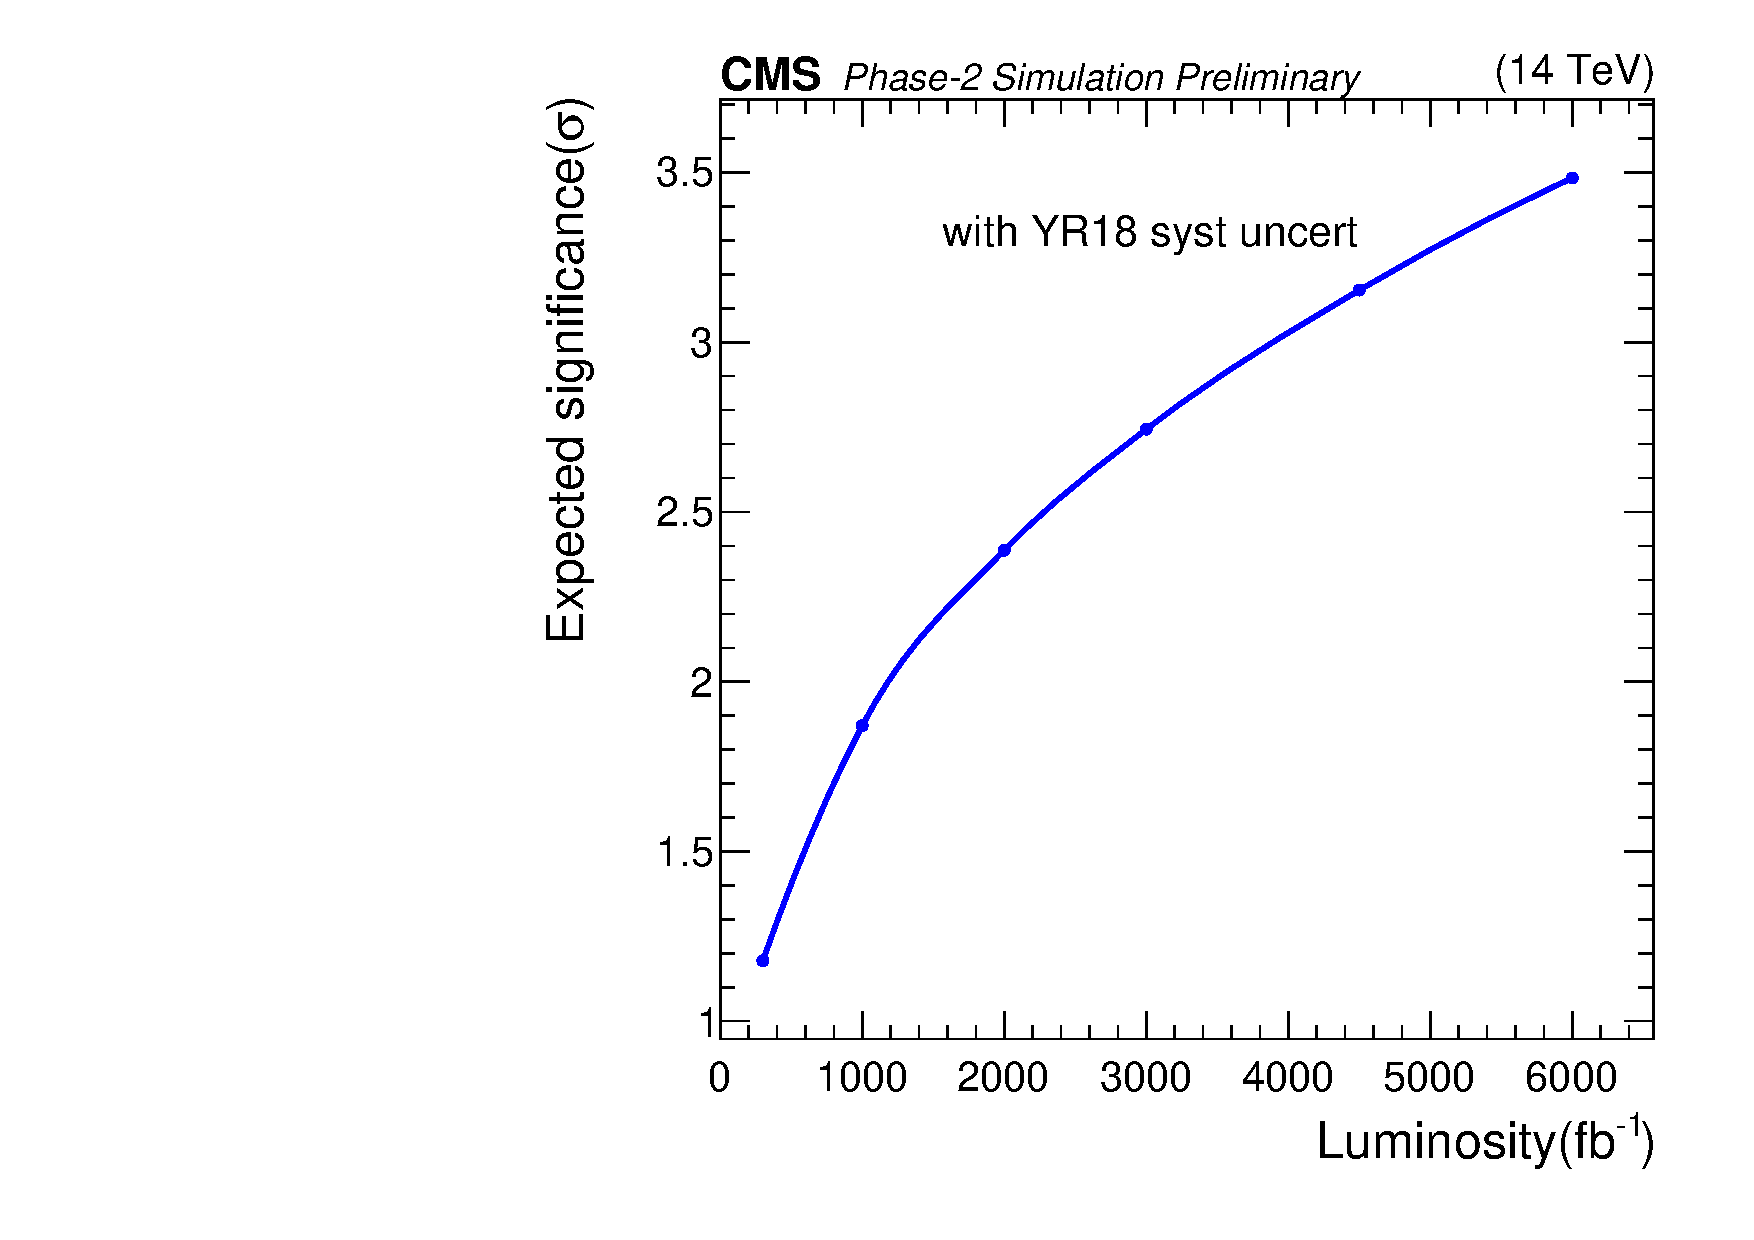
\includegraphics[width=0.32\textwidth]{CMS-PAS-FTR-18-005_Figure_007.pdf}
        }
    \subfloat[]{
        \label{fig:VBSWWFutureATLAS}
        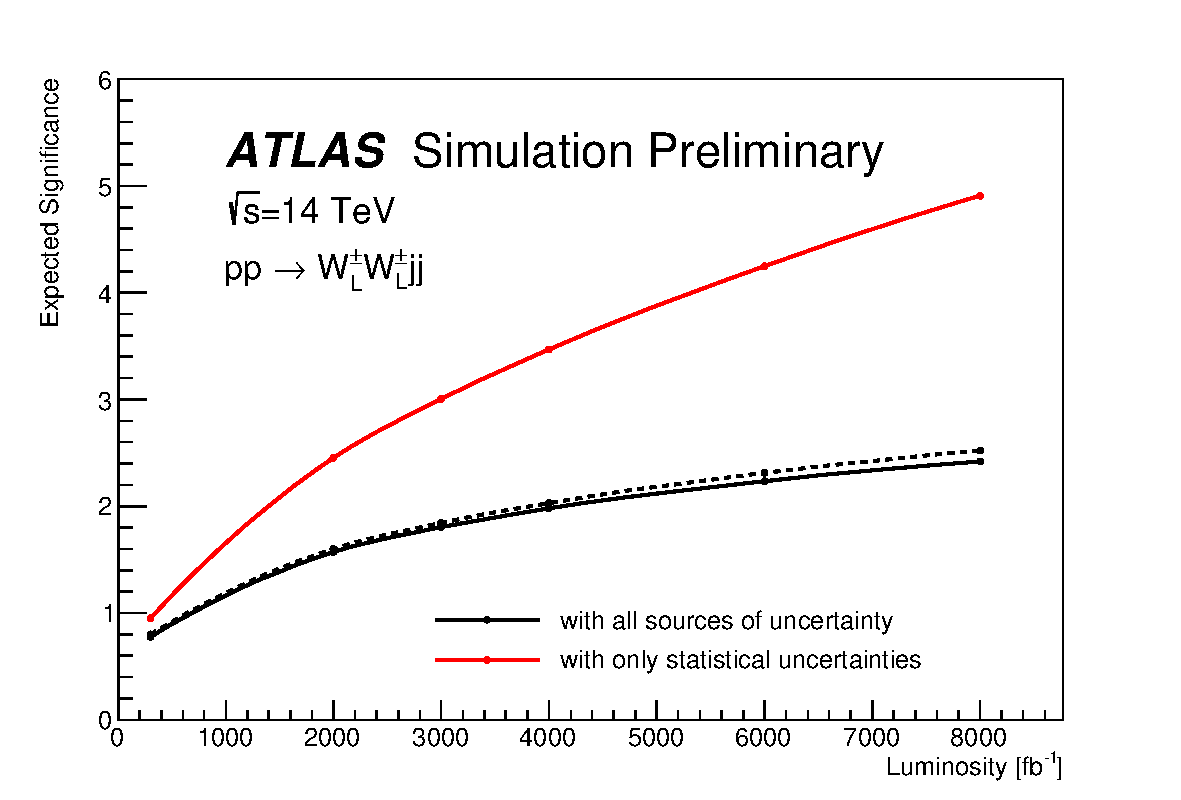
\includegraphics[width=0.48\textwidth]{fig_09.pdf}
        }
\caption{}
\label{fig:VBSWWFuture}
\end{figure}


\section{Conclusions}

A brief overview of various studies of rare processes involving multiboson interactions has been presented.
Rare processes in final states ranging from single to three boson final states are now being accessible as the integrated luminosity provided by the LHC increased dramatically over Run 1 data set.
Active usages of boosted techniques and machine learning are being deployed for better sensitivity to new physics.
We look forward to a rich interplay between theory and experiments in these final states for the Run 2 and beyond.


\begin{thebibliography}{99}
\raggedright

%%
%%  bibliographic items can be constructed using the LaTeX format in SPIRES:
%%    see    http://www.slac.stanford.edu/spires/hep/latex.html
%%  SPIRES will also supply the CITATION line information; please include it.
%%

\bibitem{Aad:2012tfa}
  G.~Aad {\it et al.}  [ATLAS Collaboration],
  ``Observation of a new particle in the search for the Standard Model Higgs boson with the ATLAS detector at the LHC,''
  Phys.\ Lett.\ B {\bf 716}, 1 (2012)
  [arXiv:1207.7214 [hep-ex]].
  %%CITATION = ARXIV:1207.7214;%%
  %3009 citations counted in INSPIRE as of 22 Jul 2014


%\cite{Chatrchyan:2012ufa}
\bibitem{Chatrchyan:2012ufa}
  S.~Chatrchyan {\it et al.}  [CMS Collaboration],
  ``Observation of a new boson at a mass of 125 GeV with the CMS experiment at the LHC,''
  Phys.\ Lett.\ B {\bf 716}, 30 (2012)
  [arXiv:1207.7235 [hep-ex]].
  %%CITATION = ARXIV:1207.7235;%%
  %2951 citations counted in INSPIRE as of 22 Jul 2014

%\cite{Weinberg:1978kz}
\bibitem{Weinberg:1978kz}
  S.~Weinberg,
  ``Phenomenological Lagrangians,''
  Physica A {\bf 96}, no. 1-2, 327 (1979).
  doi:10.1016/0378-4371(79)90223-1
  %%CITATION = doi:10.1016/0378-4371(79)90223-1;%%
  %3256 citations counted in INSPIRE as of 16 Aug 2019

%\cite{Weinberg:1979sa}
\bibitem{Weinberg:1979sa}
  S.~Weinberg,
  ``Baryon and Lepton Nonconserving Processes,''
  Phys.\ Rev.\ Lett.\  {\bf 43}, 1566 (1979).
  doi:10.1103/PhysRevLett.43.1566
  %%CITATION = doi:10.1103/PhysRevLett.43.1566;%%
  %1561 citations counted in INSPIRE as of 15 Aug 2019

%\cite{Buchmuller:1985jz}
\bibitem{Buchmuller:1985jz}
  W.~Buchmuller and D.~Wyler,
  ``Effective Lagrangian Analysis of New Interactions and Flavor Conservation,''
  Nucl.\ Phys.\ B {\bf 268}, 621 (1986).
  doi:10.1016/0550-3213(86)90262-2
  %%CITATION = doi:10.1016/0550-3213(86)90262-2;%%
  %1563 citations counted in INSPIRE as of 15 Aug 2019

%\cite{Sirunyan:2019ksz}
\bibitem{Sirunyan:2019ksz}
  A.~M.~Sirunyan {\it et al.} [CMS Collaboration],
  ``Measurement of electroweak WZ boson production and search for new physics in WZ + two jets events in pp collisions at $\sqrt{s} =$ 13TeV,''
  Phys.\ Lett.\ B {\bf 795}, 281 (2019)
  doi:10.1016/j.physletb.2019.05.042
  [arXiv:1901.04060 [hep-ex]].
  %%CITATION = doi:10.1016/j.physletb.2019.05.042;%%
  %7 citations counted in INSPIRE as of 16 Aug 2019

%\cite{deBlas:2017xtg}
\bibitem{deBlas:2017xtg}
  J.~de Blas, J.~C.~Criado, M.~Perez-Victoria and J.~Santiago,
  ``Effective description of general extensions of the Standard Model: the complete tree-level dictionary,''
  JHEP {\bf 1803}, 109 (2018)
  doi:10.1007/JHEP03(2018)109
  [arXiv:1711.10391 [hep-ph]].
  %%CITATION = doi:10.1007/JHEP03(2018)109;%%
  %33 citations counted in INSPIRE as of 16 Aug 2019

% VBS Experiment measurements
%\cite{Aad:2014zda}
\bibitem{Aad:2014zda}
  G.~Aad {\it et al.} [ATLAS Collaboration],
  ``Evidence for Electroweak Production of $W^{\pm}W^{\pm}jj$ in $pp$ Collisions at $\sqrt{s}=8$ TeV with the ATLAS Detector,''
  Phys.\ Rev.\ Lett.\  {\bf 113}, no. 14, 141803 (2014)
  doi:10.1103/PhysRevLett.113.141803
  [arXiv:1405.6241 [hep-ex]].
  %%CITATION = doi:10.1103/PhysRevLett.113.141803;%%<br />  %162 citations counted in INSPIRE as of 16 Aug 2019

%\cite{Aaboud:2019nmv}
\bibitem{Aaboud:2019nmv}
  M.~Aaboud {\it et al.} [ATLAS Collaboration],
  ``Observation of electroweak production of a same-sign $W$ boson pair in association with two jets in $pp$ collisions at $\sqrt{s}=13$ TeV with the ATLAS detector,''
  arXiv:1906.03203 [hep-ex].
  %%CITATION = ARXIV:1906.03203;%%<br />  %4 citations counted in INSPIRE as of 16 Aug 2019

%\cite{Khachatryan:2014sta}
\bibitem{Khachatryan:2014sta}
  V.~Khachatryan {\it et al.} [CMS Collaboration],
  ``Study of vector boson scattering and search for new physics in events with two same-sign leptons and two jets,''
  Phys.\ Rev.\ Lett.\  {\bf 114}, no. 5, 051801 (2015)
  doi:10.1103/PhysRevLett.114.051801
  [arXiv:1410.6315 [hep-ex]].
  %%CITATION = doi:10.1103/PhysRevLett.114.051801;%%<br />  %111 citations counted in INSPIRE as of 16 Aug 2019

%\cite{Sirunyan:2017ret}
\bibitem{Sirunyan:2017ret}
  A.~M.~Sirunyan {\it et al.} [CMS Collaboration],
  ``Observation of electroweak production of same-sign W boson pairs in the two jet and two same-sign lepton final state in proton-proton collisions at $\sqrt{s} = $ 13 TeV,''
  Phys.\ Rev.\ Lett.\  {\bf 120}, no. 8, 081801 (2018)
  doi:10.1103/PhysRevLett.120.081801
  [arXiv:1709.05822 [hep-ex]].
  %%CITATION = doi:10.1103/PhysRevLett.120.081801;%%<br />  %58 citations counted in INSPIRE as of 16 Aug 2019

%\cite{Aad:2016ett}
\bibitem{Aad:2016ett}
  G.~Aad {\it et al.} [ATLAS Collaboration],
  ``Measurements of $W^\pm Z$ production cross sections in $pp$ collisions at $\sqrt{s} = 8$ TeV with the ATLAS detector and limits on anomalous gauge boson self-couplings,''
  Phys.\ Rev.\ D {\bf 93}, no. 9, 092004 (2016)
  doi:10.1103/PhysRevD.93.092004
  [arXiv:1603.02151 [hep-ex]].
  %%CITATION = doi:10.1103/PhysRevD.93.092004;%%<br />  %102 citations counted in INSPIRE as of 16 Aug 2019

%\cite{Aaboud:2018ddq}
\bibitem{Aaboud:2018ddq}
  M.~Aaboud {\it et al.} [ATLAS Collaboration],
  ``Observation of electroweak $W^{\pm}Z$ boson pair production in association with two jets in $pp$ collisions at $\sqrt{s} =$ 13 TeV with the ATLAS detector,''
  Phys.\ Lett.\ B {\bf 793}, 469 (2019)
  doi:10.1016/j.physletb.2019.05.012
  [arXiv:1812.09740 [hep-ex]].
  %%CITATION = doi:10.1016/j.physletb.2019.05.012;%%<br />  %6 citations counted in INSPIRE as of 16 Aug 2019

%\cite{Sirunyan:2019ksz}
\bibitem{Sirunyan:2019ksz}
  A.~M.~Sirunyan {\it et al.} [CMS Collaboration],
  ``Measurement of electroweak WZ boson production and search for new physics in WZ + two jets events in pp collisions at $\sqrt{s} =$ 13TeV,''
  Phys.\ Lett.\ B {\bf 795}, 281 (2019)
  doi:10.1016/j.physletb.2019.05.042
  [arXiv:1901.04060 [hep-ex]].
  %%CITATION = doi:10.1016/j.physletb.2019.05.042;%%<br />  %7 citations counted in INSPIRE as of 16 Aug 2019

%\cite{Sirunyan:2019der}
\bibitem{Sirunyan:2019der}
  A.~M.~Sirunyan {\it et al.} [CMS Collaboration],
  ``Search for anomalous electroweak production of vector boson pairs in association with two jets in proton-proton collisions at 13 TeV,''
  arXiv:1905.07445 [hep-ex].
  %%CITATION = ARXIV:1905.07445;%%<br />  %2 citations counted in INSPIRE as of 16 Aug 2019

%\cite{Aad:2019xxo}
\bibitem{Aad:2019xxo}
  G.~Aad {\it et al.} [ATLAS Collaboration],
  ``Search for the electroweak diboson production in association with a high-mass dijet system in semileptonic final states in $pp$ collisions at $\sqrt{s}=13$ TeV with the ATLAS detector,''
  arXiv:1905.07714 [hep-ex].
  %%CITATION = ARXIV:1905.07714;%%<br />  %1 citations counted in INSPIRE as of 16 Aug 2019

%\cite{Sirunyan:2019gkh}
\bibitem{Sirunyan:2019gkh}
  A.~M.~Sirunyan {\it et al.} [CMS Collaboration],
  ``Search for anomalous triple gauge couplings in WW and WZ production in lepton + jet events in proton-proton collisions at $\sqrt{s} =$ 13 TeV,''
  arXiv:1907.08354 [hep-ex].
  %%CITATION = ARXIV:1907.08354;%%

%\cite{Sirunyan:2019dyi}
\bibitem{Sirunyan:2019dyi}
  A.~M.~Sirunyan {\it et al.} [CMS Collaboration],
  ``Measurement of electroweak production of a W boson in association with two jets in proton-proton collisions at $\sqrt{s}=$ 13 TeV,''
  arXiv:1903.04040 [hep-ex].
  %%CITATION = ARXIV:1903.04040;%%<br />  %5 citations counted in INSPIRE as of 16 Aug 2019

%\cite{CMS:2019mpq}
\bibitem{CMS:2019mpq}
  A.~M.~Sirunyan {\it et al.} [CMS Collaboration],
  ``Search for the production of W$^\pm$W$^\pm$W$^\mp$ events at $\sqrt{s} =$ 13 TeV,''
  Phys.\ Rev.\ D {\bf 100}, no. 1, 012004 (2019)
  doi:10.1103/PhysRevD.100.012004
  [arXiv:1905.04246 [hep-ex]].
  %%CITATION = doi:10.1103/PhysRevD.100.012004;%%

%\cite{Aad:2019udh}
\bibitem{Aad:2019udh}
  G.~Aad {\it et al.} [ATLAS Collaboration],
  ``Evidence for the production of three massive vector bosons with the ATLAS detector,''
  arXiv:1903.10415 [hep-ex].
  %%CITATION = ARXIV:1903.10415;%%<br />  %5 citations counted in INSPIRE as of 16 Aug 2019

%\cite{Aaboud:2018jqu}
\bibitem{Aaboud:2018jqu} 
  M.~Aaboud {\it et al.} [ATLAS Collaboration],
  ``Measurements of gluon-gluon fusion and vector-boson fusion Higgs boson production cross-sections in the $H \to WW^{\ast} \to e\nu\mu\nu$ decay channel in $pp$ collisions at $\sqrt{s}=13$ TeV with the ATLAS detector,''
  Phys.\ Lett.\ B {\bf 789}, 508 (2019)
  doi:10.1016/j.physletb.2018.11.064
  [arXiv:1808.09054 [hep-ex]].
  %%CITATION = doi:10.1016/j.physletb.2018.11.064;%%<br />  %25 citations counted in INSPIRE as of 16 Aug 2019

%\cite{Aaboud:2017vzb}
\bibitem{Aaboud:2017vzb} 
  M.~Aaboud {\it et al.} [ATLAS Collaboration],
  ``Measurement of the Higgs boson coupling properties in the $H\rightarrow ZZ^{*} \rightarrow 4\ell$ decay channel at $\sqrt{s}$ = 13 TeV with the ATLAS detector,''
  JHEP {\bf 1803}, 095 (2018)
  doi:10.1007/JHEP03(2018)095
  [arXiv:1712.02304 [hep-ex]].
  %%CITATION = doi:10.1007/JHEP03(2018)095;%%<br />  %64 citations counted in INSPIRE as of 16 Aug 2019

%\cite{ATLAS:2014aga}
\bibitem{ATLAS:2014aga} 
  G.~Aad {\it et al.} [ATLAS Collaboration],
  ``Observation and measurement of Higgs boson decays to WW$^*$ with the ATLAS detector,''
  Phys.\ Rev.\ D {\bf 92}, no. 1, 012006 (2015)
  doi:10.1103/PhysRevD.92.012006
  [arXiv:1412.2641 [hep-ex]].
  %%CITATION = doi:10.1103/PhysRevD.92.012006;%%<br />  %235 citations counted in INSPIRE as of 16 Aug 2019

%\cite{Aad:2014eva}
\bibitem{Aad:2014eva} 
  G.~Aad {\it et al.} [ATLAS Collaboration],
  ``Measurements of Higgs boson production and couplings in the four-lepton channel in pp collisions at center-of-mass energies of 7 and 8 TeV with the ATLAS detector,''
  Phys.\ Rev.\ D {\bf 91}, no. 1, 012006 (2015)
  doi:10.1103/PhysRevD.91.012006
  [arXiv:1408.5191 [hep-ex]].
  %%CITATION = doi:10.1103/PhysRevD.91.012006;%%<br />  %275 citations counted in INSPIRE as of 16 Aug 2019

%\cite{Sirunyan:2018egh}
\bibitem{Sirunyan:2018egh} 
  A.~M.~Sirunyan {\it et al.} [CMS Collaboration],
  ``Measurements of properties of the Higgs boson decaying to a W boson pair in pp collisions at $\sqrt{s}=$ 13 TeV,''
  Phys.\ Lett.\ B {\bf 791}, 96 (2019)
  doi:10.1016/j.physletb.2018.12.073
  [arXiv:1806.05246 [hep-ex]].
  %%CITATION = doi:10.1016/j.physletb.2018.12.073;%%<br />  %37 citations counted in INSPIRE as of 16 Aug 2019

%\cite{Chatrchyan:2013iaa}
\bibitem{Chatrchyan:2013iaa} 
  S.~Chatrchyan {\it et al.} [CMS Collaboration],
  ``Measurement of Higgs boson production and properties in the WW decay channel with leptonic final states,''
  JHEP {\bf 1401}, 096 (2014)
  doi:10.1007/JHEP01(2014)096
  [arXiv:1312.1129 [hep-ex]].
  %%CITATION = doi:10.1007/JHEP01(2014)096;%%<br />  %382 citations counted in INSPIRE as of 16 Aug 2019

%\cite{Sirunyan:2019twz}
\bibitem{Sirunyan:2019twz} 
  A.~M.~Sirunyan {\it et al.} [CMS Collaboration],
  ``Measurements of the Higgs boson width and anomalous $HVV$ couplings from on-shell and off-shell production in the four-lepton final state,''
  Phys.\ Rev.\ D {\bf 99}, no. 11, 112003 (2019)
  doi:10.1103/PhysRevD.99.112003
  [arXiv:1901.00174 [hep-ex]].
  %%CITATION = doi:10.1103/PhysRevD.99.112003;%%<br />  %20 citations counted in INSPIRE as of 16 Aug 2019

%\cite{Chatrchyan:2013mxa}
\bibitem{Chatrchyan:2013mxa} 
  S.~Chatrchyan {\it et al.} [CMS Collaboration],
  ``Measurement of the properties of a Higgs boson in the four-lepton final state,''
  Phys.\ Rev.\ D {\bf 89}, no. 9, 092007 (2014)
  doi:10.1103/PhysRevD.89.092007
  [arXiv:1312.5353 [hep-ex]].
  %%CITATION = doi:10.1103/PhysRevD.89.092007;%%<br />  %599 citations counted in INSPIRE as of 16 Aug 2019

%\cite{Atlas:2019qfx}
\bibitem{Atlas:2019qfx} 
  ATLAS and CMS Collaborations [ATLAS and CMS Collaborations],
  ``Report on the Physics at the HL-LHC and Perspectives for the HE-LHC,''
  arXiv:1902.10229 [hep-ex].
  %%CITATION = ARXIV:1902.10229;%%<br />  %10 citations counted in INSPIRE as of 16 Aug 2019

%% VBS Longitudinal mode unitarity
%\cite{Veltman:1976rt}
\bibitem{Veltman:1976rt} 
  M.~J.~G.~Veltman,
  ``Second Threshold in Weak Interactions,''
  Acta Phys.\ Polon.\ B {\bf 8}, 475 (1977).
  %%CITATION = APPOA,B8,475;%%
  %921 citations counted in INSPIRE as of 18 Aug 2019

%\cite{Lee:1977yc}
\bibitem{Lee:1977yc} 
  B.~W.~Lee, C.~Quigg and H.~B.~Thacker,
  ``The Strength of Weak Interactions at Very High-Energies and the Higgs Boson Mass,''
  Phys.\ Rev.\ Lett.\  {\bf 38}, 883 (1977).
  doi:10.1103/PhysRevLett.38.883
  %%CITATION = doi:10.1103/PhysRevLett.38.883;%%
  %738 citations counted in INSPIRE as of 18 Aug 2019

%\cite{Lee:1977eg}
\bibitem{Lee:1977eg} 
  B.~W.~Lee, C.~Quigg and H.~B.~Thacker,
  ``Weak Interactions at Very High-Energies: The Role of the Higgs Boson Mass,''
  Phys.\ Rev.\ D {\bf 16}, 1519 (1977).
  doi:10.1103/PhysRevD.16.1519
  %%CITATION = doi:10.1103/PhysRevD.16.1519;%%
  %2050 citations counted in INSPIRE as of 18 Aug 2019

\end{thebibliography}

